\documentclass[11pt]{article}

\usepackage[utf8]{inputenc}
\usepackage[T1]{fontenc}
\usepackage[spanish]{babel}
\usepackage{amsmath,amssymb}
\usepackage{geometry}
\usepackage{MnSymbol}

\newcommand{\s}{\mathbb{S}}
\newcommand{\N}{\mathbb{N}}
\newcommand{\im}{\text{Im}}

\geometry{margin=2.8cm}

\begin{document}

\begin{center}
    {\Large \textbf{Plan de trabajo ampliado para monografía de grado}}\\[1em]
    {\large Micaela Berezan}\\[0.5em]
    Orienta:  Juliana Xavier 
\end{center}

\vspace{1em}

La presente tiene como objetivo presentar el plan de trabajo ampliado correspondiente a
la monografía de grado de la estudiante Micaela Berezan, así como establecer un
cronograma para su desarrollo y posterior defensa.

\vspace{1em}

\section*{Temática a abordar}

% El objetivo de la monografía es estudiar diversas herramientas de topología
% algebraica y topología geométrica vinculadas a la teoría de encajes de esferas,
% con especial énfasis en la interacción entre resultados clásicos de homología y
% ejemplos de encajes salvajes en  dimensión baja.\\

En la categoría de los espacios topológicos, un encaje $f\,\colon\,\s^{n-1}\to\s^n$ es un homeomorfismo sobre su imagen, es decir, una función continua e inyectiva tal que $f^{-1}\,\colon\, \im(f)\to\s^{n-1}$ es continua. El objetivo de este trabajo es estudiar el espacio $\s^{n}-f(\s^{n-1})$.

Como primer resultado se aborda el teorema de separación de Jordan-Brouwer, que caracteriza los grupos de homología de $\s^{n}-f(\s^{k})$ para todo encaje $f$, con $n, k\in\N$. Para llegar a esto se introducen nociones básicas de homología simplicial y singular, junto con algunas herramientas y resultados clásicos que a su vez nos permitirán calcular los grupos de homología de las esferas en general.

En el caso de codimensión $1$, es decir, dada $f\,\colon\,\s^{n-1}\to\s^n$, el teorema de separación de Jordan-Brouwer garantiza que $\s^{n}-f(\s^{n-1})$ está compuesto por dos componentes conexas por caminos, y que además estas componentes son bolas homológicas. Esta última afirmación da el pie para presentar el isomorfismo de Hurewicz entre el primer grupo de homología de un espacio y el abelianizado de su primer grupo fundamental, con esto obtenemos que $\pi_1(\s^{n}-f(\s^{n-1}))$ siempre va a tener abelianizado nulo.

A continuación nos enfocamos en dar hipótesis suficientes para garantizar que las clausuras de las componentes de $\s^{n}-f(\s^{n-1})$ sean $n$-bolas. Como punto de partida para esto se prueba el teorema generalizado de Schoenflies, que garantiza que una hipótesis suficiente es que $f\,\colon\,\s^{n-1}\to\s^n$ se extienda a un encaje $\tilde{f}\,\colon\,\s^{n-1}\times [-1,1]\to\s^n$, con $\tilde{f}\,|\,_{\s^{n-1}\times\{0\}} = f$. 

Para encajes $f\,\colon\,\s^2\to\s^3$, la hipótesis de Schoenflies no puede debilitarse. Para verificar esto introducimos la noción de los entornos de collar locales para un encaje, y probamos que en general un encaje $g\,\colon\, Y\to X$ que presenta entornos de collar locales en todo punto admite un entorno de collar global, es decir, admite una extensión $\tilde{g}\,\colon\, Y\times [0,1]\to X$ con $\tilde{g}\,|\,_{Y\times\{0\}}=g$. Con este resultado reducimos la negación de la tesis del teorema generalizado de Schoenflies a una cuestión local del encaje. Esto nos permite construir un ejemplo $f\,\colon\,\s^2\to\s^3$ que presenta un único punto sin entornos de collar locales, y que además verifica que $\pi_1(\s^3 - f(\s^2))\neq 0$, confirmando que una mínima debilitación en la hipótesis ya no garantiza la tesis. 

En el caso de un encaje $f\,\colon\,\s^{n-1}\to\s^n$ con $n>3$, la hipótesis si puede debilitarse, y la manera de hacerlo es agregar puntos al conjunto $C$, conformado por los puntos de $\s^{n-1}$ que no admiten entornos de collar locales. Probaremos que si $C$ consiste de un único punto, la tesis sigue estando garantizada. Luego se presentan, sin prueba de suficiencia, las hipótesis minimales para este caso: $C$ es un conjunto de Cantor, y cumple que alguno de los dos $C\subset\s^{n-1}$ o $f(C)\subset\s^n$ está encajado de manera no estándar. Junto con esto, se describen ejemplos de encajes $f\,\colon\,\s^{n-1}\to\s^n$ con $n>3$ para los cuales $C$ y $f(C)$ son conjuntos de Cantor encajados de forma estándar, y tales que se cumple $\pi_1(\s^n-f(\s^{n-1}))\neq 0$, verificando que esta última versión de las hipótesis efectivamente sería minimal.

A la par de los resultados, se presentarán diversos ejemplos clásicos de encajes $f\,\colon\,\s^2\to\s^3$, en su mayoría cumpliendo $\pi_1(\s^3 - f(\s^2))\neq 0$, con el objetivo de exhibir distintas posibilidades para la topología del conjunto $C$, entre ellas un punto aislado, un conjunto de Cantor encajado de distintas maneras, una curva, e incluso es posible que abarque toda la esfera $\s^2$.







% Como punto de partida se introducirán las nociones básicas de homología simplicial y singular, presentando las definiciones fundamentales, ejemplos y propiedades elementales necesarias para la construcción de los grupos de homología, así como el resultado que identifica el abelianizado del grupo fundamental con el primer grupo de homología para espacios conexos por caminos. A continuación se desarrollará la sucesión exacta de Mayer-Vietoris, obtenida a partir del lema de la serpiente aplicado a una sucesión exacta de complejos de cadenas. Esta herramienta permitirá calcular la homología de las esferas y servirá como ingrediente central en la demostración del teorema de separación de Jordan-Brouwer, que se estudiará a continuación.\\


% Una vez desarrolladas estas herramientas se abordará el teorema generalizado de
% Schoenflies, siguiendo la demostración de Morton Brown, que establece que, dado
% un encaje de $S^{n}\times I$ en $S^{n+1}$, la clausura de cada componente conexa
% del complemento es una $(n+1)$-bola.\\

% Para completar el panorama de cómo se ven los encajes topológicos se presentarán resultados sobre la estructura del conjunto de puntos no localmente planos de encajes de codimensión uno en dimensión mayor que tres, en particular el teorema de Robion Kirby que describe las restricciones topológicas que debe satisfacer dicho conjunto cuando es no trivial.\\

% Finalmente, se estudiarán diversos ejemplos clásicos de encajes de $S^{2}$ en
% $S^{3}$, entre ellos la esfera de Alexander, la esfera de Antoine, la alfombra
% de Bing y la esfera de Fox-Artin. Para cada uno de estos ejemplos se describirá
% su construcción, se verificará que el espacio obtenido es una esfera topológica
% y se analizarán las propiedades de sus regiones complementarias, así como la
% naturaleza de sus puntos no localmente planos. Estos ejemplos ilustran los
% fenómenos que distinguen a los encajes salvajes de los encajes localmente planos
% y permiten apreciar el alcance de los resultados desarrollados previamente.\\

% Sugerimos el siguiente tribunal: Richard Mu\~niz, Aldo Portela y Rafael Potrie, Suplente: Juliana Xavier (orientadora).

\section*{Informe de Avance}

A continuación se listarán secciones de la monografía. Se marcarán con un asterisco las secciones que aún están en desarrollo.

\begin{itemize}
    \item Introducción a la homología
    \item Teorema de separación de Jordan-Brouwer
    \item Relación entre $H_1$ y $\pi_1$
    \item Teorema generalizado de Schoenflies
    \item Entornos de collar*
    \item Hipótesis minimales en el caso $n>3$*
    \item Ejemplos*
\end{itemize}

% \chapter{desvarios}

\begin{teo}
    Teorema de Whitehead:

    
\end{teo}



% \chapter{Homología}
\section{Homología simplicial}

\comm{agregar que una triangulación del espacio nos da una estructura de complejo simplicial}

En esta sección introduciremos al lector a la teoría de homología simplicial. Se presentarán algunas definiciones y ejemplos con el objetivo de desarrollar primeras intuiciones sobre la teoría de homología, para luego dar paso a la definición de homología singular en el siguiente capítulo. \br 

% El objetivo será probar que una $(n-1)$-esfera separa $\R^n$ en dos componentes conexas, y que estas componentes conexas tienen la misma homología de un punto. \br

Para empezar, definiremos lo que es un $n$-símplice:\br

\begin{df} Un $n$-símplice es el menor conjunto convexo de $\R^{m}\; (m\geq n)$ que contiene $n+1$ puntos $v_0,\dots,v_n$, tales que $v_1-v_0$, $v_2-v_0$, $\dots$, $v_n-v_0$ son linealmente independientes. Llamaremos vértices a estos $v_i$.\end{df}\br

En general, dado un $n$-símplice, vamos a darle un orden a sus vértices, y notaremos al símplice $[v_0,v_1,\dots,v_n]$ de acuerdo con este orden. \br

\begin{df}
Un orden en los vértices nos induce un orden en la restricción a un subconjunto de esos vértices. Haremos uso de la siguiente notación:
$$[v_0,\dots,\hat{v_i},\dots,v_n]:=[v_0,\dots,v_{i-1},v_{i+1},\dots,v_n]$$ \br
Esta es una forma de notar el $(n-1)$-símplice obtenido al sacar $v_i$ del conjunto de vértices de $[v_0,\dots,v_n]$ y tomar el menor conjunto convexo que contiene a los vértices restantes. \br

Diremos que $[v_0,\dots,\hat{v_i},\dots,v_n]$ es una cara de $[v_0,\dots,v_n]$.\br

\begin{obs}
El borde de un $n$-símplice $\Delta^n$ es la unión de sus $n+1$ caras, lo notaremos $\partial\Delta^n$. \br
\end{obs}

Llamaremos aristas a los $2$-símplices con vértices $v_i, v_j\in\{v_0,\dots,v_n\}$. Estas también heredan el orden de $[v_0,\dots,v_n]$, y por lo tanto las notamos $[v_i,v_j]$ si $i<j$.\br
\end{df}

% Al definirlo así, implícitamente le estamos dando a los vértices de $[v_0,\dots,\hat{v_i},\dots,v_n]$ el orden heredado de restringir el orden de $[v_0,\dots,v_n]$ al nuevo conjunto de vértices. \br

Como se muestra en la imagen \ref{simplices}, un ejemplo de $3$-símplice es un tetraedro en $\R^3$, un $2$-símplice es un triángulo en $\R^2$, un $1$-símplice es un intervalo en $\R$, y un $0$-símplice es un punto.\br


\begin{figure}[h!]
    \centering
    \includegraphics[width=0.5\linewidth]{img mono/simplices.png}
    \caption{$n$-símplices con las orientaciones de sus aristas, $n\in\{0,1,2,3\}$}
    \label{simplices}
\end{figure}

\comm{las imágenes no son finales, eventualmente las voy a hacer en digital}

\begin{df}
Llamaremos $n$-símplice estándar al conjunto $$\Delta^n := \Bigl\{(x_0,\dots,x_n)\in\R^{n+1} : x_i\geq 0\text{ para todo } i, \;\sum\limits_{i=0}^nx_i=1\Bigr\}$$
\end{df}

Los vértices de este $n$-símplice son los que conforman la base canónica de $\R^{n+1}$. Si notamos a estos puntos $e_1,\dots,e_{n+1}$, otra forma de escribir este conjunto es $$\Delta^n=[e_1,\dots,e_{n+1}] \subset \R^{n+1}$$\br

Para $n=2$, el $2$-símplice estándar $\Delta^2$ es el triángulo en $\R^3$ con vértices $(1,0,0)$, $(0,1,0)$ y $ (0,0,1)$. Con $n=1$, el $1$-símplice estándar es el segmento que va de $(1,0)$ a $(0,1)$ en $\R^2$. Esto se muestra en la imagen \ref{estandar}.\br

\begin{figure}[h!]
    \centering
    \includegraphics[width=0.5\linewidth]{img mono/simplices estandar.png}
    \caption{$n$-símplices estándar, $n\in\{0,1,2\}$}
    \label{estandar}
\end{figure}

\begin{df}
Dado un $n$-símplice $[v_0,\dots,v_n]$,  la función $h:\Delta^n\to [v_0,\dots,v_n]$ dada por $$h(x_0,\dots,x_n)=\sum\limits_{i=0}^n x_i v_i$$ es un homeomorfismo lineal que preserva el orden de las aristas. Llamaremos a esta función el homeomorfismo canónico.
\end{df}\br

La función $h$ es lineal y manda los elementos $e_0,\dots,e_n$ de la base canónica de $\R^{n+1}$ a $v_0,\dots, v_n$ respectivamente, por lo tanto su imagen es el $n$-símplice $[v_0,\dots,v_n]$ y el orden de las aristas se mantiene.\br

Antes de entrar en la definición de homología singular, vamos a definir la homología simplicial, que nos va a dar una imagen de las intuiciones que en la homología singular se ven más ofuscadas a cambio de obtener una teoría menos rígida y más limpia para trabajar.  \comm{cambiar este párrafo}\br

Para empezar, vamos a definir lo que será una estructura de $\Delta$-complejo para un espacio topológico cualquiera. Esto va a ser el análogo en dimensión $n$ de triangular nuestro espacio con $2$-símplices.\br


\begin{df}
    Una estructura de $\Delta$-complejo para un espacio topológico $X$ es una familia de funciones continuas $\sigma_\alpha:\Delta^{n_\alpha}\to X$ que cumplen:\br

    \begin{enumerate}
        \item Las $\sigma_\alpha$ son inyectivas al restringirlas a $Int(\Delta^{n_\alpha})$, y dado cualquier $x\in X$, existe algún $\alpha$ tal que $x$ está en la imagen de $Int(\Delta^{n_\alpha})$ por $\sigma_\alpha$.
        
        \item Si restringimos cualquier $\sigma_\alpha$ a una cara de $\Delta^{n_\alpha}$, esa restricción va a ser equivalente a otro mapa de la familia $\sigma_\beta:\Delta^{n_\alpha-1}\to X$, identificando la cara de $\Delta^{n_\alpha}$ con $\Delta^{n_\alpha-1}$ mediante el homeomorfismo canónico.

        \item Un conjunto $U\subset X$ es abierto $\iff$ $\sigma_\alpha^{-1}(U)$ es abierto para todo $\alpha$.
    \end{enumerate}
\end{df}\br

Las condiciones $(1)$ y $(3)$ nos dicen que las funciones $\sigma_\alpha$ restrictas a $Int(\Delta^{n_\alpha})$ son homeomorfismos sobre su imagen.\br

En el punto $(2)$, la equivalencia es en el siguiente sentido: \br

Dada $\sigma_\alpha:\Delta^{n_\alpha}\to X$, notamos $\hat{\Delta}^{n_\alpha}$ a una cara de $\Delta^{n_\alpha}$. Consideramos $h:\Delta^{n_\alpha -1}\to\hat{\Delta}^{n_\alpha}$ el homeomorfismo canónico que manda el $\{n_\alpha -1\}$-símplice estándar a $\hat{\Delta}^{n_\alpha}$. Lo que nos dice este punto es que existe una función $\sigma_\beta:\Delta^{n_\alpha -1}\to X$ en la familia que cumple $\sigma_\beta=\sigma_\alpha\circ h$. Decimos entonces que $\sigma_\alpha |_{\hat{\Delta}^{n_\alpha}}$ es equivalente a $\sigma_\beta$ y lo notaremos $\sigma_\alpha |_{\hat{\Delta}^{n_\alpha}}\simeq\sigma_\beta$.\br

Si por cada elemento $\sigma_\alpha:\Delta^{n_\alpha}\to X$ proveniente de la estructura de $\Delta$-complejo de $X$ consideramos un $n_\alpha$-símplice $\Delta^{n_\alpha}_\alpha$, entonces $X$ es el espacio obtenido al tomar el cociente de $x\sim h(x)$ para todas las $h:\Delta^{n_\alpha -1}\to \hat{\Delta}^{n_\alpha}_\alpha$ definidas como en el párrafo anterior. Algunos ejemplos se muestran en la imagen \ref{cocientes}.\br

\begin{figure}[h!]
    \centering
    \begin{subfigure}[]{0.4\linewidth}
        \includegraphics[width=\linewidth]{img mono/cociente.png}
    \end{subfigure}
    \begin{subfigure}[]{0.4\linewidth}
        \includegraphics[width=\linewidth]{img mono/cociente2.png}
    \end{subfigure}
    \caption{Cocientes de símplices}
    \label{cocientes}
\end{figure}

\comm{me gustaría mejorar cómo está redactado pero no quiero abusar de los subíndices, porque sería una $h$ por cada cara de cada símplice}\br

%\begin{obs}
%Cualquier espacio con una estructura de $\Delta$-complejo va a ser Hausdorff, 
%\end{obs}

%\comm{capaz decir algo más acá y poner una imagen, obs sobre hff}

\begin{df}
    Dada una estructura de $\Delta$-complejo para un espacio $X$, definimos $\dx$ como el grupo abeliano libre generado por los $\{\sigma_\alpha:\Delta^{n_\alpha}\to X \; | \; n_\alpha=n\}$. Es decir, los elementos de $\dx$, a los que llamaremos $n$-cadenas, son sumas formales finitas $\sum_{i=1}^{N} k_i\sigma_i$, con $k_i\in\N$.
\end{df}

Nuestro objetivo ahora será definir un homomorfismo de grupos $\partial_n:\dx\to\ddx$ al que llamaremos mapa borde. Para motivar la definición primero nos enfocaremos en dimensiones $2$ y $3$, consideramos entonces las caras de $\Delta^2$ y $\Delta^3$.\br

En la imagen \ref{mal orientado} se muestra la orientación usual de las caras de cada uno de estos símplices, derivada del orden en sus vértices.\br

\begin{figure}[h!]
    \centering
    \begin{subfigure}[]{0.2\linewidth}
        \includegraphics[width=\linewidth]{img mono/norient2.png}
        \caption{$[v_1,v_2]$, $[v_0,v_2]$ y $[v_0,v_1]$}
    \end{subfigure}
    \hspace{2cm}
    \begin{subfigure}[]{0.2\linewidth}
        \includegraphics[width=\linewidth]{img mono/norient4.png}
        \caption{$[v_1,v_2,v_3]$, $[v_0,v_2,v_3]$, $[v_0,v_1,v_3]$ y $[v_0,v_1,v_2]$}
    \end{subfigure}
    \caption{Orientación usual}
    \label{mal orientado}
\end{figure}

A continuación, en la imagen \ref{bien orientados} ilustramos cómo quedan orientadas las caras si revertimos la orientación de los $[v_0,\dots,\hat{v_i},\dots,v_n]$ con $i$ impar.\br

\begin{figure}[h!]
    \centering
    \begin{subfigure}[]{0.2\linewidth}
        \includegraphics[width=\linewidth]{img mono/borient2.png}
        \caption{$[v_1,v_2]$, $-[v_0,v_2]$ y $[v_0,v_1]$}
    \end{subfigure}
    \hspace{2cm}
    \begin{subfigure}[]{0.2\linewidth}
        \includegraphics[width=\linewidth]{img mono/borient4.png}
        \caption{$[v_1,v_2,v_3]$, $-[v_0,v_2,v_3]$, $[v_0,v_1,v_3]$ y $-[v_0,v_1,v_2]$}
    \end{subfigure}
    \caption{Orientación obtenida al intercalar los signos}
    \label{bien orientados}
\end{figure}

\comm{sé que el formato de las imágenes está muy feo acá, en el futuro acomodaré todo eso cuando agregue las imágenes finales}

La idea entonces es que para obtener una orientación coherente y homogénea en las caras de nuestro símplice, vamos a intercalar la orientación usual de las caras con la orientación revertida. 

\begin{df}

Procedemos ahora a definir el homomorfismo $\partial_n:\dx\to\ddx$. Para esto, fijamos su valor en los generadores de $\dx$, es decir, las funciones $\displaystyle{\sigma_\alpha:\Delta^n\to X}$. Notando $\Delta^n=[v_0,\dots,v_n]$, definimos $$\partial_n(\sigma_\alpha):=\sum\limits_{i=0}^{n}(-1)^i \sigma_\alpha|_{[v_0,\dots,\hat{v_i},\dots v_n]}$$ 

\end{df}

Definir el homomorfismo de esta manera lo dota de la siguiente propiedad, que será esencial para el desarrollo de la teoría:

\begin{lema}
La composición $\partial_{n-1}\circ\partial_n :\dx\to \Delta_{n-2}(X)$ es cero.
\end{lema}

\begin{dem}
Veamos que vale para $\sigma:\Delta^n\to X$ perteneciente a los generadores de $\dx$. La composición queda de la siguiente manera: 

$$\partial_{n-1}\circ\partial_n(\sigma)=\sum\limits_{i=0}^n(-1)^i\bigg(\sum\limits_{j<i}^n (-1)^j\sigma|_{[v_0,\dots,\hat{v_j},\dots,\hat{v_i},\dots,v_n]} + \sum\limits_{j>i}^n (-1)^{j-1}\sigma|_{[v_0,\dots,\hat{v_i},\dots,\hat{v_j},\dots,v_n]}\bigg)$$

Es importante observar que en la última sumatoria obtenemos un $(-1)^{j-1}$ en vez de un $(-1)^j$. Esto se debe a que si $j>i$, entonces el vértice $v_j$ está en el lugar $j-1$ del $(n-1)$-símplice $[v_0,\dots,\hat{v_i},\dots,v_j,\dots, v_n]$.

Usando que $\partial_n$ y $\partial_{n-1}$ son homomorfismos de grupos podemos distribuir el $(-1)^i$ y obtener que cada término de la sumatoria es de la forma $(-1)^i(-1)^j\sigma|_{[v_0,\dots,\hat{v_j},\dots,\hat{v_i},\dots,v_n]}$ si $i>j$, o $(-1)^i(-1)^{j-1}\sigma|_{[v_0,\dots,\hat{v_i},\dots,\hat{v_j},\dots,v_n]}$ si $i<j$. Dos términos se cancelan al intercambiar $i$ por $j$ y por lo tanto concluimos $\partial_{n-1}\circ\partial_n(\sigma)=0$. $\square$

\end{dem}

\begin{df}
    
Obtuvimos una familia de homomorfismos $\partial_n$ entre grupos abelianos libres $\dx$ que cumplen $\partial_{n-1}\circ\;\partial_n= 0$. Agregando un último elemento $\partial_0:\Delta_0(X)\to 0$ que definimos trivialmente, tenemos 

$$\dots\rightarrow \Delta_{n+1}(X)\xrightarrow{\partial_{n+1}}\dx\xrightarrow{\partial_n}\ddx\rightarrow\dots\rightarrow\Delta_{1}(X)\xrightarrow{\partial_1}\Delta_{0}(X)\xrightarrow{\partial_0} 0$$\br

Llamamos a una familia como esta un complejo de cadenas.

\end{df}\br

Otra forma de describir la propiedad $\partial_{n-1}\circ\;\partial_n=0$ es decir que $\im(\partial_{n+1})\subset\Ker(\partial_n)$, con esto vamos a definir los grupos de homología del complejo de cadenas.\br

\begin{df}

Definimos el $n$-ésimo grupo de homología simplicial del complejo de cadenas como el cociente $$H_n^{\Delta}(X):=\Ker(\partial_n)/\im(\partial_{n+1})$$\br

Llamamos ciclos a los elementos de $\Ker(\partial_n)$ y bordes a los de $\im(\partial_{n+1})$. Los elementos de $H_n^{\Delta}(X)$ serán nuestras clases de homología simplicial.\br 

Diremos que dos ciclos que pertenecen a la misma clase de homología simplicial son ciclos homólogos. Dos ciclos $\sum_{i=0}^N k_i\sigma_i$ y $\sum_{i=0}^M k'_i\sigma'_i$ de esta manera cumplirán que su diferencia $\sum_{i=0}^N k_i\sigma_i - \sum_{i=0}^M k'_i\sigma'_i$ es un borde.\br

\end{df}

\comm{En algún momento debería hacer una observación sobre por qué uso $\Delta$-complejos en vez de complejos simpliciales, que son los que dan el nombre a la homología simplicial. La verdad es que lo hago así porque hatcher lo hace así, y él dice que lo hace así porque los $\Delta$-complejos son más generales y más fáciles de trabajar que los simpliciales, sin embargo la verdad es que todo esto lo podría haber hecho con complejos simpliciales y no hubiera cambiado demasiado porque solo lo uso para introducir las intuiciones. O sea, \textit{mi} razón para hacerlo así es que hatcher lo hace así pero bueno debería decir algo que no sea eso.}

A continuación nos enfocaremos en algunos ejemplos.

\begin{ex}
    Comenzemos con el ejemplo más sencillo. Tomamos $X = \{p\}$ un punto. Una estructura de $\Delta$-complejo para $X$ está dada por una única función $\{\sigma_0:\Delta^0\to X\}$. \br
    
    Los grupos $\Delta_n(X)$ son $0$ salvo para $n=0$, en ese caso se tiene $\Delta_0(X)=\langle\sigma_0\rangle\simeq\Z$. Por esta razón, todos los homomorfismos $\partial_n:\dx\to\ddx$ son $0$, incluyendo $\partial_0:\Delta_0(X)\to 0$, que es $0$ por definición.\br

    Por lo tanto, en este caso tenemos $\im(\partial_n)=0$ para todo $n$, $\Ker(\partial_n)=0$ para todo $n\neq 0$, y $Ker(\partial_0)=\Delta_0(X)\simeq\Z$.\br

    Entonces $$H^{\Delta}_n(X)\simeq
    \begin{cases}
    0\text{ si } n\neq 0 \\
    \Z\text{ si } n=0
    \end{cases}$$
\end{ex}\br

\begin{ex}
Consideremos ahora $X=S^1$. Para darle una estructura de $\Delta$-complejo, vemos todo $S^1$ como una arista $e$ con un único vértice $v$ como se muestra en la imagen \ref{s1}. Nuestra estructura de $\Delta$-complejo para $X$ está dada por dos funciones $\sigma_0:\Delta^0\to X$ y $\sigma_1:\Delta^1\to X$. Si notamos $\Delta^1=[v_0,v_1]$ entonces $\im(\sigma_0)=\{v\}$, $\im(\sigma_1)=e$ y $\sigma_1|_{[v_0]}\simeq\sigma_1|_{[v_1]}\simeq\sigma_0$.\br

\begin{figure}[h!]
    \centering
    \includegraphics[width=0.3\linewidth]{img mono/s1.png}
    \caption{$S^1$}
    \label{s1}
\end{figure}

Los grupos $\dx$ son $0$ para todo $n\neq 0,1$. Para $n=1$ se tiene $\Delta_1(X)=\langle\sigma_1\rangle\simeq\Z$ y para $n=0$ se tiene $\Delta_0(X)=\langle\sigma_0\rangle\simeq\Z$.\br

Como $\sigma_1|_{[v_0]}\simeq\sigma_1|_{[v_1]}$, entonces $\partial_1(\sigma_1)=\sigma_1|_{[v_1]}-\sigma_1|_{[v_0]}=0$ y por lo tanto $\Ker(\sigma_1)=\Delta_1(X)$. Además sabemos que $\Delta_2(X)=0$ y por lo tanto $\im(\partial_2)=0$. Con esto obtenemos que $H^\Delta_1(X)\simeq\Z$.\br

En el caso de $H_0^\Delta(X)$, observamos que $\Ker(\partial_0)=\Delta_0(X)$ y $\im(\partial_1)=0$ por la misma razón que antes. Con esto obtenemos que $H^\Delta_0(X)\simeq\Z$.\br

Como $\dx=0$ para todo $n\neq 0,1$, concluimos que 

$$ H^{\Delta}_n(X)\simeq
    \begin{cases}
    0\text{ si } n\neq 0,1 \\
    \Z\text{ si } n\in\{0,1\}
    \end{cases} $$

Más adelante vamos a calcular los grupos de homología de las demás esferas.
\end{ex}

\begin{ex}

Sea $X=\T^2$, sabemos que podemos expresarlo como cociente de $[0,1]^2$. Para darle una estructura de $\Delta$-complejo, separamos $[0,1]$ en dos triángulos como se ve en la imagen \ref{toro}, que llamamos $U$ y $L$. Los bordes de estos triángulos, después de pasar por el cociente, serán nuestras tres aristas $a,b$ y $c$, que comparten un único vértice $v$. 

\begin{figure}[h!]
    \centering
    \includegraphics[width=0.3\linewidth]{img mono/toro.png}
    \caption{$\T^2$}
    \label{toro}
\end{figure}

Una estructura de $\Delta$-complejo para $X$ está dada por $\{\sigma_2^1,\sigma_2^2,\sigma_1^1,\sigma_1^2,\sigma_1^3,\sigma_0\}$, con 

$$\begin{cases}
    \sigma_2^1:\Delta^2\to U\\
    \sigma_2^2:\Delta^2\to L\\
    \sigma_1^1:\Delta^1\to a\\
\end{cases}\hspace{1cm}
\begin{cases}
    \sigma_1^2:\Delta^1\to b\\
    \sigma_1^3:\Delta^1\to c\\
    \sigma_0:\Delta^0\to \{v\}\\
\end{cases}$$

Si notamos $\Delta^2=[v_0,v_1,v_2]$, $\Delta^1=[w_0,w_1]$, entonces se cumplen las relaciones \br
$$\begin{cases}
    \sigma_2^1|_{[\hat{v_0},v_1,v_2]}\simeq\sigma_1^2\\
    \sigma_2^1|_{[v_0,\hat{v_1},v_2]}\simeq\sigma_1^3\\
    \sigma_2^1|_{[v_0,v_1,\hat{v_2}]}\simeq\sigma_1^1
\end{cases}\hspace{0.5cm}
\begin{cases}
    \sigma_2^2|_{[\hat{v_0},v_1,v_2]}\simeq\sigma_1^1\\
    \sigma_2^2|_{[v_0,\hat{v_1},v_2]}\simeq\sigma_1^3\\
    \sigma_2^2|_{[v_0,v_1,\hat{v_2}]}\simeq\sigma_1^2
\end{cases}\hspace{0.5cm}
\begin{cases}
    \sigma_1^i|_{[\hat{w_0},w_1]}\simeq\sigma_0 \\
    \sigma_1^i|_{[w_0,\hat{w_1}]}\simeq\sigma_0 
\end{cases} \fall i\in\{1,2,3\}$$\br

Observar que estas relaciones están en parte determinadas por la orientación de los símplices, esto es parte de la rigidez que impone la teoría de los $\Delta$-complejos.\br

Tenemos entonces que $\dx=0$ para todo $n\neq 0,1,2$, $\Delta_2(X)=\langle\sigma_2^1, \sigma_2^2 \rangle\simeq\Z\oplus\Z$, $\Delta_1(X)=\langle\sigma_1^1,\sigma_1^2,\sigma_1^3\rangle\simeq\Z\oplus\Z\oplus\Z$, $\Delta_0(X)=\langle\sigma_0\rangle\simeq\Z$.\br

Estudiemos primero el caso de $\partial_2$. Se tiene $\partial_2(\sigma_2^1)=\sigma_1^2-\sigma_1^3+\sigma_1^1$. Haciendo un abuso de notación, podemos escribirlo como $\partial U=b-c+a$. De la misma manera, tenemos $\partial_2(\sigma_2^2)=\sigma_1^1-\sigma_1^3+\sigma_1^2$, que podemos escribir como $\partial L=a-c+b$. Por lo tanto, continuando con esta notación, la imagen de $\partial_2$ es el grupo abeliano libre generado por $a+b-c$. Por esto mismo también obtenemos que $\Ker(\partial_2)$ es el grupo abeliano libre generado por $U-L$, que es isomorfo a $\Z$.\br

Consideramos ahora $\partial_1$. Como $\sigma_1^i|_{[\hat{w_0},w_1]}\simeq\sigma_0\simeq\sigma_1^i|_{[w_0,\hat{w_1}]}$ para $i\in\{1,2,3\}$, tenemos que $\im(\partial_1)=0$ y $\Ker(\partial_1)=\Delta_1(X)$.\br

Como $\Delta_3(X)=0$ se cumple que $im(\partial_3)=\Ker(\partial_3)=0$. Para $\partial_0$ se cumple $\im(\partial_0)=0$ y $\Ker(\partial_0)=\Delta_1(X)$ trivialmente.\br

Con esto, continuando con el abuso de notación tenemos que 
\begin{align*}
        &H^\Delta_2(X)=\Ker(\partial_2)/\im(\partial_3)\simeq\Z \\
        &H^\Delta_1(X)=\Ker(\partial_1)/\im(\partial_2)=\langle a,b,c \;|\; a+b-c=0\rangle\simeq \Z\oplus\Z \\
        &H^\Delta_0(X)=\Ker(\partial_0)/\im(\partial_1)\simeq\Z
\end{align*}

y todos los demás $H^\Delta_n(X)$ se anulan.

\comm{es posible que este ejemplo sea mucha notación}
\end{ex}
\comm{me gustaría poner algunos ejemplos más, me gustaría pegar un par de 2-símplices para mostrar cómo el borde queda solo la parte de afuera y todo lo de adentro se cancela}

\begin{obs}
    Recordar que llamamos bordes a los elementos de $\im(\partial_n)$ y ciclos a los de $\Ker(\partial_n)$. La idea detrás de estos nombres puede comenzar a aclararse observando el caso de $H^\Delta_1(X)$ para un espacio $X$ cualquiera.\br
    
    Si notamos $\Delta^1=[v_0,v_1]$ y tomamos $\sigma_i:\Delta^1\to X$ provenientes de la estructura de $\Delta$-complejo de $X$ entonces un elemento de $\Ker(\partial_1)$ es una suma formal $\sum k_i\sigma_i$ con $\sum k_i\sigma_i|_{[\hat{v_0},v_1]} - \sum k_i\sigma_i|_{[v_0,\hat{v_1}]}=0$. Un elemento de esta manera debe cumplir que cada vértice tiene el mismo número de aristas entrantes y salientes. Al ver $X$ como cociente de símplices, esto se traduce en la noción de que las imágenes de las $\sigma_i$ forman curvas cerradas.\br

    Un elemento de $\im(\partial_2)$ es también un elemento de $Ker(\partial_1)$, y por lo tanto su imagen pasada por el cociente también es unión de curvas cerradas. Sin embargo, a diferencia de los elementos de $\Ker(\partial_1)$, estas curvas cerradas necesariamente son el borde de algún $\Delta$-complejo de dimensión 2, por ejemplo de un disco.\br

    Lo que logra $H_1^\Delta(X)$ es distinguir las curvas cerradas contractibles de las no contractibles en $X$. Es decir, distingue las curvas cerradas que son borde de algún complejo de dimensión 2 de las que bordean un "agujero" en $X$. Dicho usando la nomeclatura de ciclos y bordes, los elementos relevantes para $H_1^\Delta$ son los ciclos que no son borde de ningun $2$-complejo.\br
\end{obs}

Finalmente, tiene sentido plantearnos la pregunta: Dadas dos estructuras de $\Delta$-complejo para un mismo espacio $X$, son los grupos $H^\Delta_n(X)$ isomorfos? \br

La respuesta es que si, y veremos la prueba en el siguiente capítulo.



% \section{Homología singular}

El objetivo de este capítulo será definir los grupos de homología singular de un espacio topológico $X$. Esta definición es muy similar a la vista en el capítulo anterior, con la notoria diferencia de que en vez de considerar una estructura de $\Delta$-complejo para $X$, directamente tomamos el cociente en la familia de todas las funciones $\sigma:\Delta^n\to X$.

\begin{df}
    Un $n$-símplice singular es una función continua $\sigma:\Delta^n\to X$.
\end{df}

El nombre "singular" hace referencia a que $\sigma$ no tiene por qué ser inyectiva, por lo tanto no necesariamente es un encaje. Esto significa que la imagen de $\sigma$ puede tener singularidades, es decir, puntos de autointersección. \br

\duda{acá solo dice que puede tener "sigularidades" pero no explica, yo lo interpreto así, como puntos de autointersección, pero capaz hay algo más que se me está pasando?}

\begin{df}
    Llamaremos complejo de $n$-cadenas singulares, que notaremos $C_n(X)$, al grupo abeliano libre que tiene como base a los elementos de la familia de funciones $\{\sigma:\Delta^n\to X \;\vert\; \sigma \text{ continua}\}$. \br

    Es decir, los elementos de $C_n(X)$, a los que llamaremos $n$-cadenas singulares, serán sumas formales finitas $\sum_{i=1}^k n_i\sigma_i$, con $n_i\in\Z$, y $\sigma_i:\Delta^n\to X$.
\end{df}

Comparados con su equivalente $\Delta^n(X)$ del capítulo anterior, los complejos de $n$-cadenas singulares $C_n(X)$ tienen un cardinal mucho más grande, y en la mayoría de los casos serán  grupos no numerables. \br

\begin{df}
    Definimos un mapa borde $\partial_n:\Ch\to\ch$ dado por $$\partial_n(\sigma):= \sum\limits_{i=0}^{n}(-1)^i \sigma |_{[v_0,\dots,\hat{v_i},\dots,v_n]}$$ 
    Donde estamos notando $\Delta^n$ como $[v_0,\dots,v_n]$ e identificando $[v_0,\dots,\hat{v_i},\dots,v_n]$ con $\Delta_{n-1}$ mediante el homeomorfismo canónico.
\end{df}

En algunos casos simplemente usaremos $\partial$ para notar este mapa.\br

Exactamente de la misma forma que en el capítulo anterior, obtenemos que la composición $\partial_{n-1}\circ\partial_n :C_{n}(X)\to C_{n-2}(X)$ es cero. Por lo tanto tenemos $\im(\partial_{n-1})\subset\Ker(\partial_{n})$ y podemos definir los grupos de homología singular.\br

\begin{df}
Definimos el $n$-ésimo grupo de homología singular del complejo de cadenas como el cociente $$H_n(X):=\Ker(\partial_n)/\im(\partial_{n+1})$$\br

De la misma forma que antes llamaremos ciclos a los elementos de $\Ker(\partial_n)$, bordes a los de $\im(\partial_{n+1})$ y los elementos de $H_n(X)$ serán nuestras clases de homología singular.\br 
\end{df}

Con esta definición, obtenemos trivialmente un resultado importante para la teoría.

\begin{prop}
Si $X$, $Y$ son homeomorfos, entonces $H(X)=H(Y)$
\end{prop}
\begin{proof}
Sean $h:X\to Y$ homeomorfismo. Dada $sigma:\Delta^n\to X$ continua, consideramos su composición $h\circ\sigma$
\end{proof}


% \section{Sucesión de Mayer-Vietoris}

Una familia de grupos abelianos $\{A_n:n\in \N\}$ y morfismos $\alpha_n: A_n\to A_{n-1}$ constituye una $\textbf{sucesión exacta}$ si para todo $n\in\N$ se cumple $\Ker(\alpha_{n})=\im(\alpha_{n+1})$.
\begin{obs}

La inclusión $\im(\alpha_{n+1})\subset\Ker(\alpha_{n})$ nos dice que $\alpha_{n+1}\circ\alpha_{n}\equiv 0$, es decir, los $\alpha_n$ forman un complejo de cadenas. La otra inclusión, $\im(\alpha_{n+1})\supset\Ker(\alpha_{n})$, nos dice que los grupos de homología asociados a este complejo de cadenas son triviales.

En general, podemos interpretar la sucesión de grupos de homología asociados a un complejo de cadenas como un indicador de qué tan cerca está el complejo de ser una sucesión exacta.
\end{obs}
Llamaremos \textbf{sucesión exacta corta} a una sucesión exacta de la forma $$0\rightarrow A\xrightarrow{f} B\xrightarrow{g} C\rightarrow 0$$

\begin{obs}
	Una sucesión de esta forma es exacta si y solo si $f$ es inyectiva, $g$ es sobreyectiva y $\Ker(g)=\im(f)$. Por lo tanto, $g$ induce un isomorfismo entre $C$ y $B/\im(f)$.
\end{obs}
% En general, una \textbf{sucesión exacta larga} es cualquier sucesión exacta con más términos que una sucesión exacta corta. En este capítulo, usaremos el término para referirnos específicamente a sucesiones exactas con una cantidad infinita numerable de elementos.

Sean $A$, $B$ y $C$ espacios tales que para todo $n\in\N$ tenemos morfismos $f_n\colon C_n(A)\to C_n(B)$ y $g_n\colon C_n(B)\to C_n(C)$ que constituyen una sucesión exacta corta $$0\rightarrow C_n(A)\xrightarrow{f_n} C_n(B)\xrightarrow{g_n} C_n(C)\rightarrow 0$$ y que además conmutan con los morfismos borde $\partial_n$ como en el siguiente diagrama \[\begin{tikzcd}
	& \vdots & \vdots & \vdots & \\
	0 & {C_n(A)} & {C_{n}(B)} & {C_{n}(C)} & 0 \\
	0 & {C_{n-1}(A)} & {C_{n-1}(B)} & {C_{n-1}(C)} & 0 \\
	& \vdots & \vdots & \vdots
	\arrow[from=1-2, to=2-2]
	\arrow[from=1-3, to=2-3]
	\arrow[from=1-4, to=2-4]
	\arrow[from=2-1, to=2-2]
	\arrow["{f_n}", from=2-2, to=2-3]
	\arrow["{\scriptsize\partial_n}", from=2-2, to=3-2]
	\arrow["{g_n}", from=2-3, to=2-4]
	\arrow["{\scriptsize\partial_n}", from=2-3, to=3-3]
	\arrow[from=2-4, to=2-5]
	\arrow["{\scriptsize\partial_n}", from=2-4, to=3-4]
	\arrow[from=3-1, to=3-2]
	\arrow["{f_{n-1}}"', from=3-2, to=3-3]
	\arrow[from=3-2, to=4-2]
	\arrow["{g_{n-1}}"', from=3-3, to=3-4]
	\arrow[from=3-3, to=4-3]
	\arrow[from=3-4, to=3-5]
	\arrow[from=3-4, to=4-4]
\end{tikzcd}\]

Entonces, en ese caso decimos que tenemos una \textbf{sucesión exacta corta de complejos de cadena}, que notamos $$0\rightarrow C_\bullet(A)\xrightarrow{f} C_\bullet(B)\xrightarrow{g} C_\bullet(C)\rightarrow 0$$

El foco de este capítulo es describir la existencia de una sucesión exacta particular, conocida como la Sucesión de Mayer-Vietoris. La existencia de esta sucesión va a surgir del siguiente hecho algebraico:

\begin{lema}{\emph{Lema de la serpiente}:}
	Sean $A$, $B$ y $C$ espacios que componen una sucesión exacta corta de complejos de cadena $$0\rightarrow C_\bullet(A)\xrightarrow{f} C_\bullet(B)\xrightarrow{g} C_\bullet(C)\rightarrow 0$$
	Entonces, para cada $n\in\Z$ existe un morfismo $$\partial_n^* :H_{n}(C)\rightarrow H_{n-1}(A)$$ tal que la siguiente sucesión es exacta:

$$\begin{tikzcd}[arrow style=math font,cells={nodes={text height=2ex,text depth=0.75ex}}]
       \cdots \arrow[overlay, r, "f_{n+1}^*"] & H_{n+1}(B) \arrow[overlay, r, "g_{n+1}^*"] \arrow[overlay, draw=none]{d}[name=Y, shape=coordinate]{} & H_{n+1}(C) \arrow[overlay, curarrow={Y}{\partial_{n+1}^*}]{dll}{} \\
       H_{n}(A) \arrow[overlay, r, "f_n^*"] & H_{n}(B) \arrow[overlay, r, "g_n^*"] \arrow[overlay, draw=none]{d}[name=Z,shape=coordinate]{} & H_{n}(C) \arrow[overlay, curarrow={Z}{\partial_{n}^*}]{dll}{} \\
       H_{n-1}(A) \arrow[overlay, r, "f_{n-1}^*"] & H_{n-1}(B) \arrow[overlay, r, "g_{n-1}^*"] & \cdots
\end{tikzcd}$$
\end{lema}

\begin{proof}
	Citar libro
\end{proof}

% Dado un subconjunto $Y\subset X$, consideramos la inclusión $i\colon Y\hookrightarrow X$. 

Vamos a obtener la sucesión de Mayer-Vietoris para un espacio cubierto por dos abiertos $A$ y $B$ aplicando este lema a una sucesión exacta corta de complejos de cadena en particular. Los complejos de $n$-cadenas serán los siguientes:

\begin{itemize}
	\item $C_n(A+B)$: Lo definimos como el grupo abeliano libre generado por los $n$-símplices singulares $\sigma\colon\Delta^n\to A\cup B$ tales que tienen su imagen contenida en $A$ o $B$. De esta forma, podemos verlo como subgrupo de $C_n(A\cup B)$, y entonces podemos ver el mapa borde $\partial_n^+\colon C_{n}(A + B)\to C_{n-1}(A + B)$ como la restricción de $\partial_n\colon C_n(A\cup B)\to C_{n-1}(A\cup B)$.
	\item $C_n(A\cap B)$: No hay mucho que aclarar para este complejo, salvo observar que viendo $C_n(A\cap B)$ como subgrupo de $C_n(A\cup B)$, el morfismo $\partial^\cap_n\colon C_n(A\cap B)\to C_{n-1}(A\cap B)$ puede obtenerse restringiendo $\partial_n\colon C_n(A\cup B)\to C_{n-1}(A\cup B)$.
	\item $C_n(A)\oplus C_n(B)$: Definimos el mapa borde como $\partial_n^\oplus\colon C_n(A)\oplus C_n(B)\to C_{n-1}(A)\oplus C_{n-1}(B)$ tal que $\partial_n^\oplus(a, b) = \left(\partial_n^A(a), \partial_n^B(b)\right)$, siendo $\partial_n^A\colon C_n(A)\to C_{n-1}(A)$ y $\partial_n^B\colon C_n(B)\to C_{n-1}(B)$ los respectivos mapas borde de $A$ y $B$, que pueden verse como restricción del mapa $\partial_n\colon C_n(A\cup B)\to C_{n-1}(A\cup B)$. Notaremos a este complejo $C_\bullet(A)\oplus C_\bullet(B)$.
\end{itemize}


\begin{lema}
Las inclusiones $C_n(A+B)\hookrightarrow C_n(A\cup B)$ inducen isomorfismos en los grupos de homología. $$H_n(A\cup B)\simeq H_n(A+B)$$
\end{lema}
% \[\begin{tikzcd}
% 	\dots & {C_n(A+B)} & {C_{n-1}(A+B)} & \dots \\
% 	\dots & {C_n(A\cup B)} & {C_{n-1}(A\cup B)} & \dots
% 	\arrow[from=1-1, to=1-2]
% 	\arrow[from=1-2, to=1-3]
% 	\arrow["i", hook, from=1-2, to=2-2]
% 	\arrow[from=1-3, to=1-4]
% 	\arrow["i", hook, from=1-3, to=2-3]
% 	\arrow[from=2-1, to=2-2]
% 	\arrow[from=2-2, to=2-3]
% 	\arrow[from=2-3, to=2-4]
% \end{tikzcd}\]

\comm{esta prueba creo que no la voy a agregar}

\begin{lema}
	Sean \begin{align*}
		&\psi_n\colon C_n(A\cap B)\to C_n(A)\oplus C_n(B),\quad \psi_n(x)=(x,-x) \\
		&\phi_n\colon C_n(A)\oplus C_n(B)\to C_n(A+B), \quad \phi_n(x,y)=x+y
	\end{align*}
	Entonces, la siguiente es una sucesión exacta corta de complejos de cadena:
	$$0\rightarrow C_\bullet(A\cap B)\xrightarrow{\psi}C_\bullet(A)\oplus C_\bullet(B)\xrightarrow{\phi}C_\bullet(A+B)\rightarrow 0$$
\end{lema}

% Definiendo $\psi_n(x)=(x,-x)$, $\phi_n(x,y)=x+y$ consideramos el siguiente diagrama:

% $$0\rightarrow C_n(A\cap B)\xrightarrow{\psi_n}C_n(A)\oplus C_n(B)\xrightarrow{\phi_n}C_n(A+B)\rightarrow 0$$

% Esta va a resultar una sucesión exacta corta, vamos a verificarlo.
\begin{proof}

Los $\psi_n$, $\phi_n$ son morfismos para cada $n\in\N$. Lo que falta verificar es que las sucesiones son exactas para cada $n$ y que los morfismos conmutan con el mapa borde. Veamos primero que dado $n\in\N$, la siguente sucesión es exacta: $$0\rightarrow C_n(A\cap B)\xrightarrow{\psi_n}C_n(A)\oplus C_n(B)\xrightarrow{\phi_n}C_n(A+B)\rightarrow 0$$

\begin{itemize}

\item $\Ker(\phi_n)\subset\im(\psi_n)$: Si se cumple $(x,y)\in\Ker(\phi_n)$ para dos elementos $x\in C_n(A)$, $y\in C_n(B)$, entonces se cumple $x+y=0$. Esto implica que $y=-x$ como cadenas en $A\cup B$, y por lo tanto $x, y\in C_n(A\cap B)$. Tenemos entonces $\psi_n(x)=(x,-x)=(x,y)\in C_n(A)\oplus C_n(B)$, es decir, $(x,y)\in\im(\psi_n)$. 

\item $\im(\psi_n)\subset\Ker(\phi_n)$: Dado $(x,-x)\in\im(\psi_n)$ se tiene $x\in C_n(A\cap B)$, entonces $\phi_n(x,-x)=x-x=0$

\item $\Ker(\psi_n)=0$: Dado $x\in C_n(A\cap B)$ tal que $\psi_n(x)=0$, se tiene $(x,-x)=(0,0)$ en $C_n(A)\oplus C_n(B)$, entonces $x=0$.

\item $\im(\phi_n)=C_n(A+B)$: Dado $x\in C_n(A+B)$, $x$ es una suma formal de $n$-símplices singulares con imagen contenida en $A$ o $B$. Veamos que todos los generadores están contenidos en la imagen de $\phi_n$, y con eso obtenemos $\im(\phi_n)=C_n(A+B)$. Sea $\sigma_A:\Delta^n\to A\cup B$ un $n$-símplice singular con imagen contenida en $A$, entonces la suma formal compuesta por el único elemento $\sigma_A$ es imagen por $\phi_n$ del elemento $(i\circ\sigma_A ,0)\in C_n(A)\oplus C_n(B)$, con $i\colon A\hookrightarrow A\cap B$ la inclusión. Análogamente tenemos lo mismo para un símplice con imagen contenida en $B$.
 
% \comm{observacion sobre def del neutro en el grupo libre}

\end{itemize}
Con esto concluimos que la sucesión es exacta. Ahora resta verificar que los morfismos conmutan con el borde, es decir, que los siguientes diagramas conmutan:

% https://q.uiver.app/#q=WzAsOCxbMCwwLCJcXHNjcmlwdHN0eWxlIENfbihBXFxjYXAgQikiXSxbMSwwLCJcXHNjcmlwdHN0eWxlIENfbihBKVxcb3BsdXMgQ19uKEIpIl0sWzEsMSwiXFxzY3JpcHRzdHlsZSBDX3tuLTF9KEEpXFxvcGx1cyBDX3tuLTF9KEIpIl0sWzAsMSwiXFxzY3JpcHRzdHlsZSBDX3tuLTF9KEFcXGNhcCBCKSJdLFsyLDAsIlxcc2NyaXB0c3R5bGUgQ19uKEEpXFxvcGx1cyBDX24oQikiXSxbMiwxLCJcXHNjcmlwdHN0eWxlIENfe24tMX0oQSlcXG9wbHVzIENfe24tMX0oQikiXSxbMywwLCJcXHNjcmlwdHN0eWxlIENfbihBK0IpIl0sWzMsMSwiXFxzY3JpcHRzdHlsZSBDX3tuLTF9KEErQikiXSxbMSwyLCJcXHNjcmlwdHN0eWxlIFxccGFydGlhbF9uXlxcb3BsdXMiXSxbMCwzLCJcXHNjcmlwdHN0eWxlIFxccGFydGlhbF9uXlxcY2FwIl0sWzAsMSwiXFxzY3JpcHRzdHlsZSBcXHBzaV9uIiwyXSxbMywyLCJcXHNjcmlwdHN0eWxlIFxccHNpX3tuLTF9Il0sWzQsNSwiXFxzY3JpcHRzdHlsZSBcXHBhcnRpYWxfbl5cXG9wbHVzIl0sWzQsNiwiXFxzY3JpcHRzdHlsZVxccGhpX24iLDJdLFs1LDcsIlxcc2NyaXB0c3R5bGUgXFxwaGlfe24tMX0iXSxbNiw3LCJcXHNjcmlwdHN0eWxlXFxwYXJ0aWFsX25eKyIsMl1d
\[\begin{tikzcd}
	{\scriptstyle C_n(A\cap B)} & {\scriptstyle C_n(A)\oplus C_n(B)} & {\scriptstyle C_n(A)\oplus C_n(B)} & {\scriptstyle C_n(A+B)} \\
	{\scriptstyle C_{n-1}(A\cap B)} & {\scriptstyle C_{n-1}(A)\oplus C_{n-1}(B)} & {\scriptstyle C_{n-1}(A)\oplus C_{n-1}(B)} & {\scriptstyle C_{n-1}(A+B)}
	\arrow["{\scriptstyle \psi_n}"', from=1-1, to=1-2]
	\arrow["{\scriptstyle \partial_n^\cap}", from=1-1, to=2-1]
	\arrow["{\scriptstyle \partial_n^\oplus}", from=1-2, to=2-2]
	\arrow["{\scriptstyle\phi_n}"', from=1-3, to=1-4]
	\arrow["{\scriptstyle \partial_n^\oplus}", from=1-3, to=2-3]
	\arrow["{\scriptstyle\partial_n^+}"', from=1-4, to=2-4]
	\arrow["{\scriptstyle \psi_{n-1}}", from=2-1, to=2-2]
	\arrow["{\scriptstyle \phi_{n-1}}", from=2-3, to=2-4]
\end{tikzcd}\]
% \begin{align*}
% \psi_{n-1}\circ\partial_n &=\psi_n\circ\partial_n \\
% \phi_{n-1}\circ\partial_n &=\phi_n\circ\partial_n
% \end{align*}

Empezamos verificando la condición del diagrama de la izquierda. Sea $x\in C_n(A\cap B)$, entonces
\begin{align*}
	\partial_n^\oplus \circ\psi_n(x)&=\partial_n^\oplus (x,-x)=\left(\partial_n^A(x), \partial_n^B(-x)\right) = \left(\partial_n(x),\partial_n(-x)\right) = \left(\partial_n(x),-\partial_n(x)\right)\\
	&= \psi_{n-1}\circ \partial_n(x) =\psi_{n-1}\circ\partial_n^\cap(x)
\end{align*}
Ahora verifiquemos la condición del segundo diagrama. Sea $(x,y)\in C_n(A)\oplus C_n(B)$, entonces
\begin{align*}
	\partial_n^+\circ\phi_n (x,y) &= \partial_n^+(x+y)=\partial_n(x+y)\\
	&=\partial_n(x)+\partial_n(y) = \phi_{n-1}(\partial_n(x),\partial_n(y)) = \phi_{n-1}\circ\partial_n^\oplus (x,y)
\end{align*}
Con esto concluimos que tenemos una sucesión exacta corta de complejos de cadena.
\end{proof}

Combinando los tres lemas anteriores, a partir de la sucesión exacta corta de complejos de cadena 
$$0\rightarrow C_\bullet(A\cap B)\xrightarrow{\psi}C_\bullet(A)\oplus C_\bullet(B)\xrightarrow{\phi}C_\bullet(A + B)\rightarrow 0$$ 

logramos construir la siguiente sucesión exacta larga, a la que llamaremos \textbf{sucesión de Mayer-Vietoris} para los abiertos $A$ y $B$:

$$\begin{tikzcd}[arrow style=math font,cells={nodes={text height=2ex,text depth=0.75ex}}]
       \cdots \arrow[overlay, r, "\psi_{n+1}^*"] & H_{n+1}(A)\oplus H_{n+1}(B) \arrow[overlay, r, "\phi_{n+1}^*"] \arrow[overlay, draw=none]{d}[name=Y, shape=coordinate]{} & H_{n+1}(A\cup B) \arrow[overlay, curarrow={Y}{\partial_{n+1}^*}]{dll}{} \\
       H_{n}(A\cap B) \arrow[overlay, r, "\psi_n^*"] & H_{n}(A)\oplus H_{n}(B) \arrow[overlay, r, "\phi_n^*"] \arrow[overlay, draw=none]{d}[name=Z,shape=coordinate]{} & H_{n}(A\cup B) \arrow[overlay, curarrow={Z}{\partial_{n}^*}]{dll}{} \\
       H_{n-1}(A\cap B) \arrow[overlay, r, "\psi_{n-1}^*"] & H_{n-1}(A)\oplus H_{n-1}(B) \arrow[overlay, r, "\phi_{n+1}^*"] & \cdots
\end{tikzcd}$$

% \comm{acá después también voy a agregar la relación con el teo de van kampen}

También podemos obtener una sucesión de Mayer-Vietoris para homología reducida, tomando la versión aumentada de cada complejo de cadenas. Aumentar los complejos de cadenas es tomar los morfismos \begin{align*}
&\varepsilon^\cap\colon C_{0}(A\cap B)\to\Z \\
&\varepsilon^\oplus\colon C_{0}(A)\oplus C_{0}(B)\to\Z\oplus\Z\\
&\varepsilon^+\colon C_{0}(A+B)\to\Z\end{align*}

\comm{esto lo defino en la parte anterior}

% Vamos a tomar morfismos para continuar la sucesión exacta corta de complejos de cadena $0\rightarrow C_\bullet(A\cap B)\xrightarrow{\psi}C_\bullet(A)\oplus C_\bullet(B)\xrightarrow{\phi}C_\bullet(A+B)\rightarrow 0$ 
Consideramos la sucesión exacta corta $$0\rightarrow\Z\xrightarrow{\psi_{-1}}\Z\oplus\Z\xrightarrow{\phi_{-1}}\Z\rightarrow 0$$
Dada por los morfismos \begin{align*}
&\psi_{-1}\colon\mathbb{Z}\to\mathbb{Z}\oplus\mathbb{Z},\quad \psi_{-1}(x)=(x,-x)\\
&\phi_{-1}\colon\mathbb{Z}\oplus\mathbb{Z}\to\mathbb{Z},\quad\phi_{-1}(x,y)=x+y
\end{align*} 
% https://q.uiver.app/#q=WzAsMyxbMCwwLCJcXHNjcmlwdHNpemVcXG1hdGhiYntafSJdLFsxLDAsIlxcc2NyaXB0c2l6ZVxcbWF0aGJie1p9XFxvcGx1c1xcbWF0aGJie1p9Il0sWzIsMCwiXFxzY3JpcHRzaXplXFxtYXRoYmJ7Wn0iXSxbMCwxLCJcXHNjcmlwdHNpemVcXHBzaV97LTF9Il0sWzEsMiwiXFxzY3JpcHRzaXplXFxwaGlfey0xfSJdXQ==
% \[\begin{tikzcd}
% 	{\scriptsize\mathbb{Z}} & {\scriptsize\mathbb{Z}\oplus\mathbb{Z}} & {\scriptsize\mathbb{Z}}
% 	\arrow["{\scriptsize\psi_{-1}}", from=1-1, to=1-2]
% 	\arrow["{\scriptsize\phi_{-1}}", from=1-2, to=1-3]
% \end{tikzcd}\] 

Si los mapas $\varepsilon$ conmutan con los $\psi_{-1}$ y $\phi_{-1}$, entonces tenemos una sucesión exacta corta de complejos de cadena aumentados, y aplicando el lema de la serpiente obtenemos la sucesión de Mayer-Vietoris para homología reducida.

\begin{ex}
Calcular la homología de las esferas
\end{ex}
Calculemos los grupos de homología de una esfera $\s^n$. La cubrimos por abiertos $A=\s^n - \{N\}$ y $B:=\s^n - \{S\}$, siendo $N$ y $S$ los puntos norte y sur de la esfera. Los $A$ y $B$ son discos abiertos y por lo tanto su homología reducida es $0$. También cumplen que su intersección retrae por deformación a $\s^{n-1}$.

% \comm{mencionar en el cap 1 que retraer por def induce isomorfismos en los grupos de homologia}

Consideramos la versión reducida de la sucesión de Mayer-Vietoris para $A$ y $B$, pasando por los respectivos isomorfismos en los grupos de homología:

$$\begin{tikzcd}[arrow style=math font,cells={nodes={text height=2ex,text depth=0.75ex}}]
       \cdots \arrow[overlay, r, ""] & 0 \arrow[overlay, r, ""] \arrow[overlay, draw=none]{d}[name=Y, shape=coordinate]{} & \tilde{H}_{i+1}(\s^n) \arrow[overlay, curarrow={Y}{\partial_{i+1}^*}]{dll}{} \\
       \tilde{H_{i}}(\s^{n-1}) \arrow[overlay, r, ""] & 0 \arrow[overlay, r, ""] \arrow[overlay, draw=none]{d}[name=Z,shape=coordinate]{} & \tilde{H_{i}}(\s^n) \arrow[overlay, curarrow={Z}{\partial_{i}^*}]{dll}{} \\
       \tilde{H}_{i-1}(\s^{n-1}) \arrow[overlay, r, ""] & 0 \arrow[overlay, r, ""] & \cdots
\end{tikzcd}$$

Como esta sucesión es exacta, obtenemos que los $\partial^*_i$ son isomorfismos y entonces $H_i(\s^n)\cong H_{i-1}(\s^{n-1})$ para todo $i\in\N$.

Lo único que necesitamos es calcular la homología de alguna esfera en concreto, por ejemplo $\s^0$. Como $\s^0$ tiene dos componentes conexas y ambas son puntos, sabemos que su homología es 
\begin{align*}H_i(\s^0)\cong
\begin{cases}
\Z\oplus\Z \quad&\text{si }\,i=0\\
0 \quad &\text{en cualquier otro caso}
\end{cases}
\end{align*} que tomando homología reducida es lo mismo pero con $\overset{\sim}{H_0}(\s^0)\cong\Z$.

Aplicando los isomorfismos para cada $i,\, n\in\N$ tenemos
\begin{align*}\tilde{H}_i(\s^n)\cong
\begin{cases}
\Z\quad&\text{si }\,i=0,\, n\\
0 \quad &\text{en cualquier otro caso}
\end{cases}
\end{align*}

\comm{agregar tablita}

% % https://q.uiver.app/#q=WzAsMTMsWzAsMSwiMCJdLFsxLDEsIlxcc2NyaXB0c3R5bGUgQ197MH0oQVxcY2FwIEIpIl0sWzIsMSwiXFxzY3JpcHRzdHlsZSBDX3swfShBKVxcb3BsdXMgQ197MH0oQikiXSxbMywxLCJcXHNjcmlwdHN0eWxlIENfezB9KEErQikiXSxbNCwxLCIwIl0sWzAsMiwiMCJdLFs0LDIsIjAiXSxbMSwyLCJcXG1hdGhiYntafSJdLFsyLDIsIlxcc2NyaXB0c3R5bGUgXFxtYXRoYmJ7Wn1cXG9wbHVzXFxtYXRoYmJ7Wn0iXSxbMywyLCJcXG1hdGhiYntafSJdLFszLDAsIlxcdmRvdHMiXSxbMiwwLCJcXHZkb3RzIl0sWzEsMCwiXFx2ZG90cyJdLFswLDFdLFsxLDIsIlxcc2NyaXB0c2l6ZVxccHNpXzAiXSxbMiwzLCJcXHNjcmlwdHNpemVcXHBoaV8wIl0sWzMsNF0sWzksNl0sWzgsOSwiXFxzY3JpcHRzaXplXFxwaGlfey0xfSIsMl0sWzcsOCwiXFxzY3JpcHRzaXplXFxwc2lfey0xfSIsMl0sWzUsN10sWzEsNywiXFxzY3JpcHRzaXplXFxwYXJ0aWFsX24iXSxbMiw4LCJcXHNjcmlwdHNpemVcXHBhcnRpYWxfbiJdLFsxMCwzXSxbMTEsMl0sWzEyLDFdLFszLDksIlxcc2NyaXB0c2l6ZVxccGFydGlhbF9uIl1d
% \[\begin{tikzcd}
% 	& \vdots & \vdots & \vdots & \\
% 	0 & {\scriptstyle C_{0}(A\cap B)} & {\scriptstyle C_{0}(A)\oplus C_{0}(B)} & {\scriptstyle C_{0}(A+B)} & 0 \\
% 	0 & {\mathbb{Z}} & {\scriptstyle \mathbb{Z}\oplus\mathbb{Z}} & {\mathbb{Z}} & 0
% 	\arrow[from=1-2, to=2-2]
% 	\arrow[from=1-3, to=2-3]
% 	\arrow[from=1-4, to=2-4]
% 	\arrow[from=2-1, to=2-2]
% 	\arrow["{\scriptsize\psi_0}", from=2-2, to=2-3]
% 	\arrow["{\scriptsize\partial_n}", from=2-2, to=3-2]
% 	\arrow["{\scriptsize\phi_0}", from=2-3, to=2-4]
% 	\arrow["{\scriptsize\partial_n}", from=2-3, to=3-3]
% 	\arrow[from=2-4, to=2-5]
% 	\arrow["{\scriptsize\partial_n}", from=2-4, to=3-4]
% 	\arrow[from=3-1, to=3-2]
% 	\arrow["{\scriptsize\psi_{-1}}"', from=3-2, to=3-3]
% 	\arrow["{\scriptsize\phi_{-1}}"', from=3-3, to=3-4]
% 	\arrow[from=3-4, to=3-5]
% \end{tikzcd}\]


% \comm{en algún lugar de acá mencionar eso de que la sucesión de grupos de homología es una forma de expresar qué tan cerca de ser exacta está la sucesión de grupos abelianos}

% \begin{lema}
    
%     Sea $X$ un espacio topológico y $\mathcal{U}=\{U_j\}$ una familia de subespacios tales que $\{\mathring{U_j}\}$ es un cubrimiento de $X$. 

%     Definimos como $C_n^{\mathcal{U}}(X)$ al subgrupo de $C_n(X)$ dado por las cadenas $\sum_i n_i\sigma_i$

% \end{lema}

% https://q.uiver.app/#q=WzAsMTYsWzAsMSwiMCJdLFsxLDEsIkNfbihBKSJdLFsyLDEsIkNfe259KEIpIl0sWzMsMSwiQ197bn0oQykiXSxbNCwxLCIwIl0sWzAsMiwiMCJdLFs0LDIsIjAiXSxbMSwyLCJDX3tuLTF9KEEpIl0sWzIsMiwiQ197bi0xfShCKSJdLFszLDIsIkNfe24tMX0oQykiXSxbMSwzLCJcXHZkb3RzIl0sWzIsMywiXFx2ZG90cyJdLFszLDMsIlxcdmRvdHMiXSxbMywwLCJcXHZkb3RzIl0sWzIsMCwiXFx2ZG90cyJdLFsxLDAsIlxcdmRvdHMiXSxbMCwxXSxbMSwyLCJmX24iXSxbMiwzLCJnX24iXSxbMyw0XSxbOSw2XSxbOCw5LCJnX3tuLTF9IiwyXSxbNyw4LCJmX3tuLTF9IiwyXSxbNSw3XSxbMSw3LCJcXHNjcmlwdHNpemVcXHBhcnRpYWxfbiJdLFsyLDgsIlxcc2NyaXB0c2l6ZVxccGFydGlhbF9uIl0sWzMsOSwiXFxzY3JpcHRzaXplXFxwYXJ0aWFsX24iXSxbNywxMF0sWzgsMTFdLFs5LDEyXSxbMTMsM10sWzE0LDJdLFsxNSwxXV0=


% \section{Suspensión de ejemplos}

Dado un espacio $X$, llamamos \textbf{cono de X} y notamos $C(X)$ al espacio cociente obtenido a partir de $X\times[0,1]$ al colapsar $X\times\{1\}$ a un punto. Llamamos \textbf{base del cono} al conjunto $X\times\{0\}$.

Llamamos \textbf{suspensión de X} y notamos $\Sigma(X)$ al cociente obtenido a partir de $X\times [0,1]$ al colapsar $X\times\{0\}$, $X\times\{1\}$ a puntos distintos. Equivalentemente, podemos pensarlo como el pegado de dos conos por la base.

Dada una función $f:X\to Y$, notamos $\Sigma f$ a la \textbf{suspensión de} $f$. La suspensión de $X$ e $Y$ me induce una función $\Sigma f:\Sigma(X)\to\Sigma(Y)$, que es el cociente de $f\times\id:X\times[0,1]\to Y\times[0,1]$ obtenido colapsando $(X,\{0\}),(X,\{1\}),(Y,\{0\}),(Y,\{1\})$ a puntos distintos.

Veamos que si el complemento de la imagen de un encaje $h:\s^n\to\s^{n+1}$ tiene $\pi_1$ no trivial, entonces la suspensión de $\Sigma h$ cumple lo mismo.

\begin{obs}
La suspensión de una esfera $\s^n$ es $\Sigma(\s^n)\simeq\s^{n+1}$. Viendo la suspensión como dos conos pegados por la base, esto es directo de observar que $C(\s^n)\simeq \D^{n+1}$.
\end{obs}

\comm{digo algo más?}

Entonces para un encaje $h:\s^n\to\s^{n+1}$, la suspensión es nuevamente un encaje $\Sigma h:\s^{n+1}\to\s^{n+2}$. 

Calculemos $\pi_1\left(\s^{n+2}-\im(\Sigma h)\right)$, llamemos $X$ a $\im(\Sigma h)$:

$$\Sigma\,\s^{n+1} - \im(\Sigma h)\simeq \big(\s^{n+1}\times[0,1]\big)_{/\sim} - \big(h(\s^n)\times [0,1]\big)_{/\sim}$$

Como $h(\s^n)$ es no vacío, los extremos de las suspensiones se cancelan

$$\big(\s^{n+1}\times\{0,1\}\big)_{/\sim} - \big(h(\s^n)\times\{0,1\}\big)_{/\sim}=\varnothing$$

Entonces tenemos 

$$\Sigma\,\s^{n+1} - \im(\Sigma h)\simeq \big(\s^{n+1}-h(\s^n)\big)\times (0,1)$$

Por lo tanto el complemento $\big(\s^{n+1}-h(\s^n)\big)\times (0,1)$ retrae por deformación a $\s^{n+1}-h(\s^n)$.

En todo esto no estoy usando ninguna propiedad del encaje $h$. En general vale que $\s^{n+1}-\Sigma(D)$ retrae por deformación a $\s^n -D$.

% Para calcular su $\pi_1$ usamos el teorema de Van Kampen, en este caso vamos a obviar las hipótesis sobre descomposiciones conformadas por más de dos abiertos:

% \begin{teo}
% Dado $X=A\cup B$ unión de abiertos con $A$, $B$, $A\cap B$ conexos por caminos, tenemos el isomorfismo $\pi_1(X)\simeq \pi_1(A)\ast\pi_1(B)/[i_{AB},i_{BA}] $
% \end{teo}



% \comm{digo que van kampen es un pushout?}
\comm{usar MV para ver que la suspensión me hace un shift en los grupos de homología}
%\comm{corolario 4.24 Hatcher}




% \section{Un ejemplo de Alexander}

\comm{Davenma y Venema}

\comm{En la claim 2.1.5 usar la descomposición de heegaard de $\R^3$ como dos toros}

\comm{Al final de los ejemplos hablar de que tomar suspensión me da ejemplos de dim superior. Esto está en DV después de Alexander.}

En esta sección vamos a dar un ejemplo de una bola encajada en $\R^3$ tal que el encaje no se extiende a un homeomorfismo de todo $\R^3$. 

Podemos construir la imagen como una intersección numerable de cerrados encajados $\{X_n\}$. Para el resto de la construcción, va a ser conveniente definir los siguientes conjuntos auxiliares: 

Sea $T$ un toro sólido en $\R^3$ dado por un encaje $\varphi :\s^1\times \D^2\rightarrow \R^3$ y sea $[t_1,t_2]\subset \s^1$ un intervalo cerrado. Llamamos $\textbf{cilindro contenido en T}$ al conjunto $C:=\varphi([t_1,t_2]\times \D^2)$, y decimos que los dos discos $\varphi(\{t_1\}\times\D^2)$, $\varphi(\{t_2\}\times\D^2)$ son las \textbf{tapas del cilindro}.

Dado un cilindro $C$, lo que nos va a interesar en general es considerar dos toros sólidos $T'$ y $T''$ que estén contenidos en $C$, enlazados entre ellos (con un enlace simple) y con $T'\cap \partial C=\tau_1$, $T''\cap \partial C=\tau_2$ como en la imagen $\ref{alex1}$. Llamaremos $\textbf{toros enlazados en C}$ a dos toros que cumplen lo anterior.

\comm{los toros tienen número de enlace 1, ver si defino número de enlace o cómo digo eso. todos los enlaces que voy a usar siempre van a ser simples, o sea van a tener número de enlace 1. seguro esta construcción se puede hacer con número de enlace arbitrario y tiene pinta que quedan no equivalentes}

\begin{figure}[h!]
    \centering
    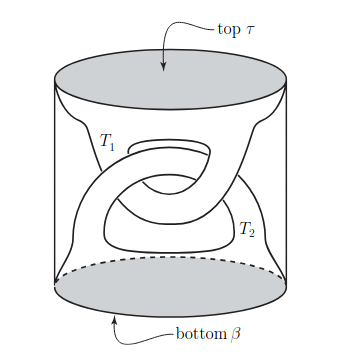
\includegraphics[width=0.5\linewidth]{img mono/alexander/1.png}
    \caption{Un cilindro conteniendo $T_1$ y $T_2$}
    \label{alex1}
\end{figure}

Ahora si, vamos a definir nuestra sucesión de cerrados encajados: 

Empezamos por $X_0$ un toro sólido estándar en $\R^3$, con diámetro menor a $1$. Consideramos un cilindro $C$ contenido en $X_0$ con diámetro menor a $\frac{1}{2}$, y llamamos $T_0$ y $T_1$ a dos toros enlazados en $C$. Definimos $X_1:=(X_0-C)\cup T_0\cup T_1$.

Para definir $X_2$, vamos a modificar sólamente los toros $T_0$ y $T_1$, y lo haremos de la misma forma en la que modificamos el toro $X_0$ en el paso anterior. Lo que hacemos es considerar dos cilindros $C_0\subset T_0$ y $C_1\subset T_1$, esta vez teniendo en cuenta que estos cilindros no intersecten a las tapas del cilindro anterior $C$, y que además tengan diámetros menores a $\frac{1}{4}$. Dentro de cada uno de estos cilindros consideramos dos toros enlazados, $T_{00}, T_{01}\subset C_0$ y $T_{10}, T_{11}\subset C_1$. Definimos $X_2$ como $$X_2:=\big[X_1-(C_0\cup C_1)\big]\cup\bigg(\bigcup\limits_{i,j\in\{0,1\}} T_{ij}\bigg)$$

El resto de la sucesión lo definimos inductivamente. Asumamos que en el paso $n$ se eliminaron los $2^{n-1}$ cilindros $\{\tilde{C_\alpha} : \alpha\in \{0,1\}^{n-1}\}$ de diámetro menor a $2^{-(n-1)}$ y se reemplazaron por los $2^n$ toros sólidos $\{T_\beta : \beta\in \{0,1\}^{n}\}$. 

Lo primero que hacemos para definir $X_{n+1}$ es considerar un cilindro $C_\beta$ contenido en cada $T_\beta$. Procuramos que este $C_\beta$ tenga diámetro menor a $2^{-n}$ y que no intersecte las tapas del cilindro $\tilde{C_\alpha}$ en el que $T_\beta$ estaba contenido.

Ahora para cada $\beta\in\{0,1\}^n$ consideramos $T_{\beta 0}$ y $T_{\beta 1}$ dos toros enlazados en $C_\beta$. Identificamos $\beta 0$ y $\beta 1$ con los elementos de $\{0,1\}^{n+1}$ que coinciden con $\beta$ en los primeros $n$ lugares y son $0$ o $1$ en el último, respectivamente.

Definimos entonces $X_{n+1}$ como $$X_{n+1}:=\bigg[X_n-\bigg(\bigcup\limits_{\beta\in\{0,1\}^n} C_\beta \bigg)\bigg]\cup\bigg( \bigcup\limits_{\gamma\in\{0,1\}^{n+1}}T_\gamma\bigg)$$

Llamamos a $B=\bigcap\limits_{n=1}^\infty X_n$ la \textbf{bola de Alexander}.

\duda{acá hay un detalle que no dije que es que los subtoros enlazados hay que tomarlos con cuidado para que después pueda considerar un cilindro contenido en cada uno con el diámetro acotado como quiero. si tomara los subtoros super gordos no me sirve aa}

% Llamamos $S=\partial B$ la esfera de Alexander. 

Veamos que $\pi_1(B^c)$ es no trivial: Tomamos $J$ una curva cerrada que sea no trivial en el complemento del toro $X_0$. Supongamos $J$ es trivial en $B^c$ y consideramos su homotopía $H$ a un punto. 
            
El conjunto $\im(H)$ es un compacto contenido en $B^c$. Observar que $B^c$ cumple $$B^c=\left(\bigcap\limits_{n=1}^\infty X_n\right)^c=\bigcup\limits_{n=1}^\infty X_n^c$$ 
Como $\{X_n^c\}$ cubre $\im(H)$, entonces existe un subcubrimiento finito $\{X_1^c,\dots, X_N^c\}$ para algún $N\in\N$. Observar que todos los $\{X_n\}$ son cerrados y cumplen $X_{n+1}\subset X_n$. Por lo tanto, la familia $\{X_n^c\}$ está compuesta por abiertos encajados. Por esta razón podemos reducir el subcubrimiento $\{X_1^c,\dots, X_N^c\}$ a uno compuesto únicamente por el elemento $X_N^c$. 

Encontramos entonces un $N\in\N$ tal que $\im(H)\subset X_N^c$, es decir, $J$ es contractible en $X_N^c$. Por inducción podemos ver que esto es absurdo. 

Ahora veamos que $B$ es una 3-célula: Pensemos $B$ como unión de cosas en vez de intersección. 

En la etapa $n$ de la construcción tenemos $2^{n-1}$ pillboxes, que cada una contiene 2 toros sólidos. Tenemos entonces $2^n$ toros sólidos en la etapa $n$, que son cada uno unión de una pillbox y una 3-célula complementaria. 

Definimos $D_n$ a la unión de las $2^{n-1}$ 3-células complementarias a las $2^{n-1}$ pillboxes en la etapa $n$ de la construcción. 

De esta manera podemos definir $B$ como $\overline{\bigcup\limits_{n=1}^\infty C_n}$, siendo $C_1=D_1$ y $C_n=C_{n-1}\cup D_n$ 
            
\duda{convencerme de por qué preciso clausurar--> $B$ es intersección arbitraria de cerrados entonces es cerrado, los $C_n$ son abiertos entonces su unión va a ser abierta. Como $B$ no es $\varnothing$ ni $\R^3$ no puede ser un clopen, entonces no son iguales. Falta convencerme pq clausurar funciona.} 

Llamemos $P_n^i$ a la i-ésima pillbox del n-ésimo paso de la construcción. Es decir, $P_n^i\subset X_n \fall i\in\{1,\dots,2^{n-1}\}$ y $X_n=X_{n+1}\cup\bigcup\limits_{i=1}^{2^{n-1}}P_n^i$. 
            
Sea $x\in B-\bigcup\limits_{n=1}^\infty C_n \Rightarrow x\in \bigcap\limits_{n=1}^\infty X_n-\bigcup\limits_{n=1}^\infty C_n$ 

$x\not\in\bigcup\limits_{n=1}^\infty C_n \Rightarrow x\not\in C_n\fall n\in\N$ 

$x\in B-C_n\Rightarrow \exst i\in\{1,\dots,2^{n-1}\}$ tal que $x\in P_n^i$ 

Con esto concluimos que $x\in B-\bigcup\limits_{n=1}^\infty C_n \Leftrightarrow x\in\bigcap\limits_{n=1}^\infty P_n^{k_n}$ para alguna sucesión de naturales $\{k_n\}$. \comm{recordar que $diam(P_n)\xrightarrow{n} 0$, son compactas y encajadas}

Como $diam(P_n)\xrightarrow{n} 0$, esto además implica que $x\in\overline{\bigcup\limits_{n=1}^\infty C_n}$, y por lo tanto tenemos la igualdad de conjuntos. 

Además, fun fact, observar que dada una pillbox $P_n^i$ se cumple que $\#\big\{j\in\{1,\dots, 2^n\}:P_{n+1}^j\cap P_n^i\neq\varnothing\big\}=2$, por lo tanto, los $x\in B-\bigcup\limits_{n=1}^\infty C_n$ están en biyección con $2^{\N}$, es decir, son un Cantor. 

Viendo $B$ de esta manera, probemos que efectivamente es una bola: 

Para cada $C_n$ en la construcción, podemos definir un homeo $h_n:C_n\to C_{n+1}$ soportado en un entorno $U_n$ de $C_n\cap D_{n+1}$. 

Definimos entonces una familia de funciones $\{f_n:C_1\to C_{n+1}\}_{n\in\N}$ tales que $f_n=h_n\circ h_{n-1}\circ\dots\circ h_1$. Observar que cada $f_n$ difiere de $f_{n+1}$ sólamente en $U_n$.

Como $diam(P_n)\xrightarrow n 0$, podemos ir tomando los $U_n$ con $diam(U_n)\xrightarrow n 0$, por lo tanto $\{f_n\}$ converge uniformemente a $f:C_1\to B$, que resulta continua. \comm{acomodar esto pq en realidad los $U_n$ son disconexos entonces el diametro no tiende a 0}

Queremos verificar ahora que $f$ es biyectiva, y con eso obtener que es un homeomorfismo. 

Por lo visto anteriormente, sabemos que $K=f^{-1}(B-\bigcup\limits_{n=1}^{\infty}C_n)$ es un conjunto de Cantor. 

Dado $x\in C_1- K$, $\exst N\in\N$ tal que $f_{N-1}(x)\in C_{N}-U_N$ (en este caso pensamos $f_0$ como la identidad), y por lo tanto $f(x)=f|_{N-1}(x)$. 
            
Con esto tenemos que $f$ es biyectiva en $C_1- K$. 

Por lo observado anteriormente, dados $x_0, x_1\in K$, en algún momento van a estar en distintas componentes conexas de los entornos $U_n$, y por lo tanto van a diferir sus imágenes por alguna de las $f_n$. Con esto tenemos la inyectividad de $f$ en $K$. 

Para la sobreyectividad, tomamos un punto $x\in B-\bigcup\limits_{n=1}^{\infty}C_n$ y su correspondiente elemento de $2^\N$, y observamos que se corresponde a un único punto \comm{terminar de escribir}


% \chapter{Schoenflies}

\comm{Agregar: Toda variedad compacta con borde tiene entorno collar.

Las clausuras de las componentes del complemento cuando no son variedades se llaman crumpled cubes, y bing prueba que un crumpled $n$-cube siempre es un retracto de $R^n$, esto implica q son contractibles.

Puede pasar q las dos componentes sean crumpled cubes, x ejemplo agarras la esfera de alexander y le pones cuernos para el otro lado tb. también hay una prueba de q agarrar la esfera y hacerle el doubling queda $S^3$}

\cite{mbsch}

% La idea de la prueba es empezar asumiendo que una de las componentes es una variedad $A$, y en ese caso encontrar un entorno de collar para $A$. Teniendo ese entorno uno se considera un disco $D_1$ qu eesté contenido en $\partial A\times [0,1]\subset A$. Tomamos $D_2=S^n-D_1$ y se cumple que $D_2\simeq \D^n$. La idea después es probar que el homeo $D_2\simeq \D^n$ se extiende a un homeo $A\simeq \D^n$, esta es la parte que lleva más trabajo, la meat and potato de la prueba.

% \begin{figure}
%     	\centering
%     	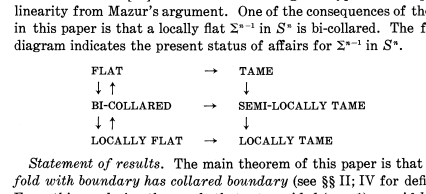
\includegraphics[width=0.5\linewidth]{img mono/schoenflies/equiv.png}
%     	\caption{M. Brown, Locally flat imbeddings of topological manifolds}
% \end{figure}

Decimos que una variedad $M^m$ está encajada en el interior de $N^n$ de forma \textbf{localmente plana} si para todo $x\in\mathring{M}$ existe un entorno $U_x$ de $N$ que contiene a $x$ y un homeomorfismo $\phi\colon U_x\to \R^n$ tal que $\phi(U_x\cap M) = \R^m$. 

\begin{lema}\label{lema1}
    Sea $f:D\to \s^n$ una función continua, siendo $D$ un disco $D\simeq \D^n$. Llamamos $X=\{x\in\s^n :\# f^{-1}(x)> 1\}$ a los puntos donde $f$ no es inyectiva. Suponemos que $X$ es finito y $f^{-1}(X)$ está contenido en el interior de $D$.

    Entonces, si $\s^n - f(\partial D)= D_1\sqcup D_2$, se cumple una de las dos opciones:

    \begin{itemize}
        \item $f(D)=D_1\cup f(\partial D)$
        \item $f(D)=D_2\cup f(\partial D)$
    \end{itemize}
\end{lema}

\begin{proof}

    Llamamos $h:=f|_{\partial D}$. Como $f^{-1}(X)\cap D=\varnothing$, $h$ es inyectiva. Con eso $h$ es continua e inyectiva entre espacios métricos compactos, entonces es un homeo sobre su imagen. Por el teorema de separación de Jordan-Brouwer, $h(\partial D)$ separa $\s^n$ en dos componentes conexas (y estas componentes son bolas homológicas, aunque no vamos a usar eso en este caso). Llamamos a estas componentes $D_1$ y $D_2$ como en el enunciado.

    En principio tenemos dos opciones:

    \begin{itemize}
        \item $f(D)\subset f(\partial D)$
        \item $f(\mathring{D})$ intersecta $D_1\sqcup D_2$
    \end{itemize}
    
    Supongamos $f(D)\subset f(\partial D)$. En ese caso podríamos considerar la composición $h^{-1}\circ f$. Esta sería una función continua que fija $\partial D$ y manda $D$ en $\partial D$, esto es absurdo. 
    
    \comm{escribir esto con más detalle?}

    Obtuvimos entonces que $f(D)$ intersecta por lo menos a una de las regiones $D_1$, $D_2$. Sin pérdida de generalidad suponemos $f(D)\cap D_1=\varnothing$.

    Sabemos que $\partial D$ no separa $D$, y $f(\partial D)$ si separa $\s^n$. Como $f^{-1}(X)\subset\mathring{D}$, entonces $f$ cumple $f(\mathring{D})\cap f(\partial D)=\varnothing$. Como $f$ es continua, manda componentes conexas en componentes conexas, y como $f(\partial D)$ separa $\s^n$ en dos componentes, entonces $f(\mathring{D})$ va a estar contenida en $D_1$.

    Por el teorema de separación de Jordan Brouwer además tenemos que $f(\partial D)=\partial D_1=\partial D_2$. Por lo tanto concluimos que $f(D)\subset \overline{D_1}$.

    Probemos ahora la otra inclusión. Si nos restrinigmos a los puntos en $D-f^{-1}(X)$, $f$ es continua e inyectiva, entonces por el teorema de invariancia del dominio la imagen por $f$ del abierto $\mathring{D}-f^{-1}(X)$ es un abierto de $\s^n$. Como $f(\partial D)=\partial D_1$, los únicos posibles puntos de $\partial(f(D))$ en el interior de $D_1$ son exactamente los elementos de $X$, que son una cantidad finita.

    Supongamos por absurdo que $\overline{D_1}\not\subset f(D)$. En ese caso, los puntos en $D_1$ se separan en tres tipos:

    % \begin{itemize}
    %     \item $x\in \overline{D_1}\cap f(\mathring{D})$
    %     \item $x\in \overline{D_1}\cap f(\partial D)$
    %     \item $x\in \overline{D_1} - f(D)$
    % \end{itemize}

    % Como $f(\partial D)=\partial D_1$ y $f^{-1}(X)\cap\partial D=\varnothing$, entonces en realidad vale

    \begin{itemize}
        \item $x\in D_1\cap \mathring{f(D)}$
        \item $x\in D_1\cap \partial f(D)$
        \item $x\in D_1 - f(D)$
    \end{itemize}

    Como $D$ es compacto y $f$ es continua entonces $f(D)$ es un compacto en $\s^n$ y por lo tanto es cerrado. Entonces los conjuntos $D_1\cap \mathring{f(D)}$ y $D_1 - f(D)$ son abiertos disjuntos. Como $D_1$ es abierto y conexo, un subconjunto que lo separe en dos componentes conexas necesariamente debe tener una cantidad infinita de puntos. Esto es absurdo, ya que antes observamos que $D_1\cap \partial(f(D))$ tiene cardinal finito.

    Con esto concluimos que $f(D)=\overline{D_1}$, probando el lema.
\end{proof}

%\comm{ahora una prueba como la gente aver}

% Idea de la prueba: Dado un encaje $\phi:\s^{n-1}\to\s^n$, consideramos $D$ la clausura de una componente de $\s^n - \phi(\s^{n-1})$. Queremos probar que si $D$ es una variedad, entonces $D\simeq \D^n$.

% Si $D$ es una variedad con borde, el borde tiene un entorno homeomorfo a $\s^{n-1}\times [0,1]$ en $D$. Llamamos $\hat{\phi}:\s^{n-1}\times [0,1]\to\s^n$ al encaje, que es una extensión de $\phi$.

% Sean $X, Y$ las dos componentes de $\s^n-\hat{\phi}(\s^{n-1}\times [0,1])$ tal que $X\subset D$. Vamos a ver que existe un mapa sobreyectivo $f:\s^n\to\s^n$ tal que manda $X$, $Y$ en dos puntos distintos $x$, $y$, y es inyectiva en $\s^n-X\cup Y$. Una vez tenemos eso, restringiendo $f$ a $D$ tenemos como imagen un disco $\D\subset\s^n$.

% La clave para esto es probar que bajo estas hipótesis $D$ cumple $D\simeq D/X$. Más específicamente, $D$ va a ser un $\textbf{conjunto celular}$.

\begin{df}
    Un subconjunto $X$ de una $n$-variedad es $\textbf{celular}$ si para todo abierto $U$ que contiene a $X$ existe una familia de conjuntos $\{D_i,i\in\N\}$ tales que 
    
    \begin{itemize}
        \item $X=\cap_{i=1}^\infty D_i$
        \item $D_i\simeq\D$, $D_i\subset U$ para todo $i\in\N$
        \item Los $D_i$ están encajados: $D_{i+1}\subset\mathring{D_i}$
    \end{itemize}
\end{df}

\begin{obs}
    Los $D_i$ son compactos, como la variedad es Hausdorff, entonces son cerrados. Por lo tanto $X$ necesariamente es cerrado.
\end{obs}

\begin{df}

    Sea $M$ una $n$-variedad compacta con borde, $X_1,\dots,X_k$ subconjuntos cerrados y disjuntos dos a dos. Llamamos $\textbf{colapsar}$ $X_1,\dots ,X_k$ en $M$ a considerar el espacio cociente $M'=M/ \sim $ dado por $x\sim x'\iff \{x,x'\}\subset X_i$ para algún $i\in\{1,\dots,k\}$.

\end{df}

Algo interesante de los conjuntos celulares es que al colapsarlos obtenemos una variedad homeomorfa a la que teníamos originalmente.

\begin{lema}\label{colapsar}
    Sea $M$ una $n$-variedad compacta con borde, $X$ subconjunto celular de $\mathring{M}$. Entonces el espacio $M'$ obtenido al colapsar $X$ es homeomorfo a $M$.
\end{lema}
\begin{proof}
    Tenemos $X=\bigcap\limits^{\infty} D_i$, con $D_i$ discos encajados como en la definición. Construyamos un mapa sobreyectivo $f:M\to M$ tal que $f|_{M-X}$ es inyectiva y $f(X)=x_0$ para algún $x_0\in M$. Este mapa va a ser el límite de una sucesión de homeos que construimos inductivamente, empezando por $f_1:= \text{Id}$.

    Para definir $f_{k+1}$, vamos a asumir que ya tenemos definido un homeo $f_k$. Lo modificamos de la siguiente manera:

    Vamos a elegir un homeomorfismo auxiliar $\hat{g}_{k+1}:f_k(D_k)\to f_k(D_k)$ tal que 
    
    \begin{itemize}
        \item $\hat{g}_{k+1}|_{\partial(f_k(D_k))}\equiv Id$
        \item $\diam\big(\hat{g}_{k+1}(f_k(D_{k+1}))\big)<\frac{1}{k+1}$
    \end{itemize}

    \comm{para el primer punto, entiendo que se está usando que el mapping class group de $\D^n$ es trivial, para poder "isotopar" $f_k|_{\partial D_k}$ a $\text{Id}$.}
    
    Una vez tenemos eso, lo extendemos a un homeo $g_{k+1}:M\to M$ como $g_{k+1}\equiv \text{Id}$ afuera de $f_k(D_k)$. Definimos $f_{k+1}:= g_{k+1}\circ f_k$.
    
%    Por ser un homeo, $f_k$ va a cumplir:

%    \begin{itemize}
%        \item $f_k(D_k)\simeq f_k(D_{k+1})\simeq\D^n$
%        \item $f_k(D_{k+1})\subset\mathring{f(D_k)}$
%    \end{itemize}

    Ahora hay que verificar que la familia de funciones $\{f_k\}$ converge punto a punto. Veamos que la sucesión $f_k(p)$ converge para todo $p\in M$. Para esto separamos en los casos $p\in X$, $p\in M-X$.

    Veamos el caso $p\in X$. Se tiene $f_k(p)\in f_k(D_k)$ para todo $k\in\N$. Por construcción, las $f_k$ cumplen 
    
    \begin{itemize}
    \item $f_1(D_1)\supset f_2(D_2)\supset f_3(D_3)\supset\dots$
    \item $\lim\limits_{k\to\infty}\text{diam}(D_k)=0$
    \end{itemize}
    Por lo tanto, la intersección $\bigcap\limits^\infty f_k(D_k)$ consiste de un único punto $x_0$, y se cumple que $\lim\limits_{k\to\infty}f_k(p)=x_0$.

    Tomemos ahora $p\in M-X$. Como los $D_k$ están encajados y $p\not\in\cap_{k=1}^\infty D_k$, existe un $K\in\N$ tal que $p\not\in D_k$ para todo $k\geq K$. Por lo tanto, la sucesión $f_k(p)$ es constante a partir de $K$.

    Con esto tenemos que las $f_k$ convergen puntualmente, llamamos $f$ al límite.

    Sabemos que $f$ es continua por definición, y que $f^{-1}(x_0)=X$. Verifiquemos que $f$ es inyectiva en $M-X$ y sobreyectiva.

    Para probar que $f$ es sobreyectiva, vamos a ver que alcanza todo elemento de $M$. Ya sabemos que $f(X)=\{x_0\}$, entonces basta verificar que un punto arbitrario $x\in M-\{x_0\}$ está en la imagen de $f$. Efectivamente, si $x\in M-\{x_0\}$ entonces $x\not\in \cap^\infty_{k=1} f_k(D_k)$, y por lo tanto a partir de un $K\in\N$ se tiene $x\not\in f_K(D_K)$, entonces $f_K^{-1}(x)\cap D_K=\varnothing$. Luego la sucesión $f_k(x)$ es constante a partir de $K$, y se cumple que $f(f^{-1}_K(x))=f_K(f^{-1}_K(x))=x$, por lo tanto $x$ está en la imagen de $f$.

    Ahora veamos que $f$ es inyectiva en $M-X$. Para eso tomamos dos puntos $x\neq y\in M-X$. Como no están en $X$, las sucesiones $f_k(x), f_k(y)$ son eventualmente constantes, y por lo tanto podemos encontrar un $K\in\N$ tal que $f(x) = f_K(x)$, $f(y) = f_K(y)$. Como $f_K$ es un homeo y $x\neq y$, entonces $f(x)\neq f(y)$.

    Con esto tenemos que $f:M\to M$ baja al cociente como una biyección continua, que además va a ser un homeo porque va de un espacio compacto a uno Hausdorff.
\end{proof}

Inductivamente obtenemos el mismo resultado para un espacio con finitos conjuntos celulares disjuntos dos a dos.

\begin{cor}\label{colapsar2}
Sea $M$ una $n$-variedad compacta con borde, sean $X_1,\dots,X_n$ subconjuntos celulares de $\mathring{M}$ disjuntos dos a dos. Entonces el espacio $M'$ obtenido al colapsar $X_1,\dots,X_n$ es homeomorfo a $M$.
\end{cor}

\begin{proof}
    Lo único que nos falta observar para usar inductivamente el lema anterior es que dados dos conjuntos celulares disjuntos $X_1$ y $X_2$, el conjunto $X_2$ sigue siendo celular en $M/\sim$ al colapsar $X_1$.

    En efecto, esto se cumple. Como $M$ es un espacio métrico, dados dos cerrados disjuntos tengo entornos disjuntos. Dados dos abiertos disjuntos de $X_1$ y $X_2$, estos van a seguir siendo abiertos en $M/_{\sim}$ al pasar por la proyección, entonces $\pi(X_2)\subset M/_{\sim}$ es celular.
    
    \comm{terminar de escribir esto, hacer la cadena de implicaciones para concluir que $M$ es metrizable y así poder usar que tengo los entornos disjuntos. o sea no es directo de ser $n$-variedad que tienen entornos que separan conjuntos pero si se puede probar, en particular $M$ admite una métrica y todo espacio metrico va a cumplir lo q buscamos.}
\end{proof}

Para poder usar esta propiedad tan útil sobre los conjuntos celulares, va a ser necesario un criterio que nos permita identificarlos. Para eso vamos a dar una definición que nos permite distinguir los subconjuntos en los que una función es inyectiva.

\begin{df}
Dada una función $f:X\to Y$, llamamos \textbf{conjunto preimagen no trivial} a los subconjuntos de $X$ que cumplen $Z=f^{-1}(y_0)$ para algún $y_0\in Y$ y tienen $\#Z > 1$.
\end{df}\comm{también podría llamarle \textbf{fibra no trivial}?}\duda{pregunta pra juliana}

% \begin{lema}
%     Sean $X_1,\dots, X_m\subset\mathring{\D}^n$ cerrados disjuntos. Sea $M/_{\sim}$ el espacio obtenido al colapsar $X_1,\dots, X_m$ y sea $\pi:M\to M/_{\sim}$ la proyección.
% \end{lema}

\begin{lema}\label{celulares}
    Sea $f:\D^n\to \s^n$ continua, sea $M\subset \mathring{\D^n}$ el único conjunto preimagen no trivial de $f$. Entonces, $M$ es un conjunto celular en $\D^n$
\end{lema}

\begin{proof}
    Por Jordan-Brouwer tenemos que $h(\partial\D^n)$ separa $\s^n$ en dos regiones. Por otro de los lemas anteriores (ordenar bien) tenemos que $h(\D^n)=h(\partial\D^n)\cup D$ siendo $D$ una de esas dos regiones.

    Tomamos un abierto $U$ que contenga a $M$. Como $f$ es inyectiva en $\D^n-M$ y es continua, entonces $f|_{\D^n-M}$ es un homeo, y por lo tanto $f(U)$ es abierto.

    Tomamos $h:\s^n\to\s^n$ un homeo que mande $\overline{D}$ en $f(U)$ y tal que $h=\text{Id}$ en un entorno $V$ de $x_0$. \comm{dice que el entorno tiene que ser chico, ver bien pq}

    Definimos $g:\D^n\to\D^n$ como $$ g(x)=
    \begin{cases}
    x \quad &\text{si } x\in M\\ 
    f^{-1}\circ h\circ f(x)\quad &\text{si } x\not\in M
    \end{cases}$$

    Como $h=\text{Id}$ en $f^{-1}(V)$ tenemos que $g$ es un homeo.

    Concluimos que $M$ es celular porque $g^k(\D^n)\subset g^{k-1}(\D^n)$ van a ser discos que aproximan $f^{-1}(V)$.
\end{proof}

\duda{me falta el paso de por qué aproximar $f^{-1}(V)$ es suficiente. creo que más bien la idea es que puedo ir definiendo $g_k$ con los entornos $V$ cada vez más chicos y ahí eee. claro creo q ya entendi. el entorno $U$ del principio es arbitrario y me consegui un disco adentro. }

\comm{insertar bien la referencia}

\begin{figure}
    	\centering
    	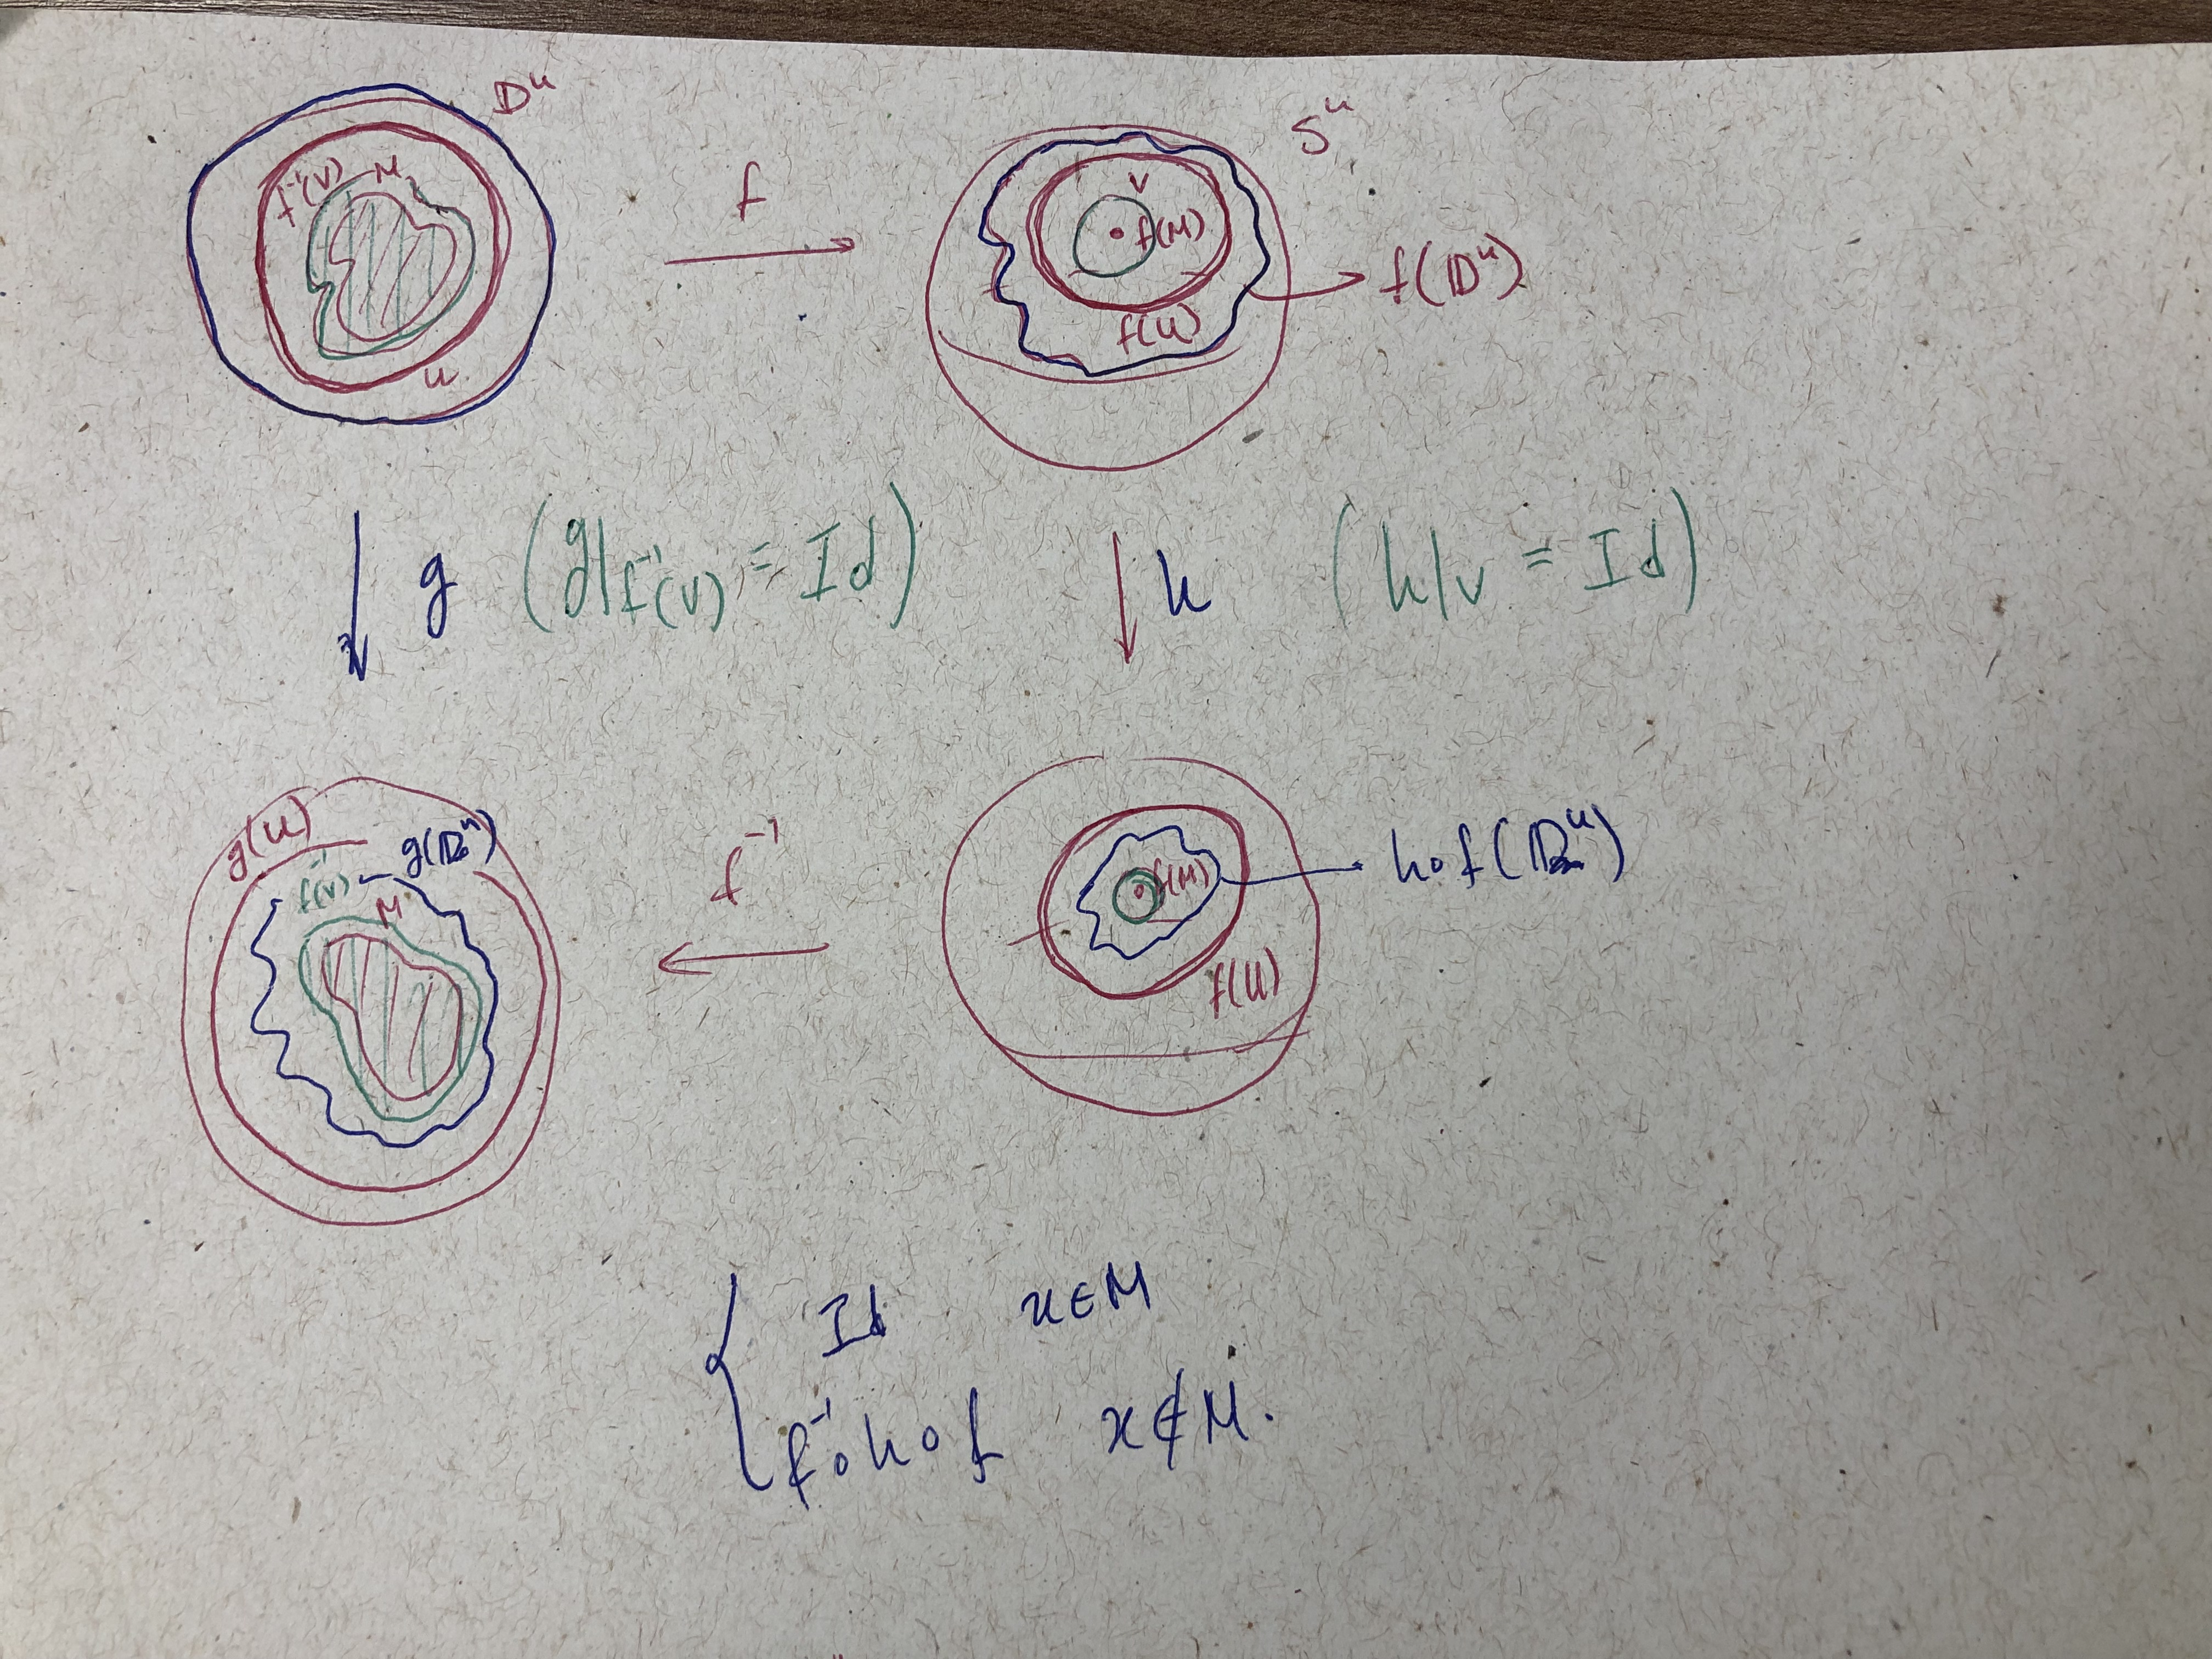
\includegraphics[width=0.75\linewidth]{img mono/schoenflies/sch.jpeg}
    	\caption{Dibujito}
        \label{dibujo1}
\end{figure}

\begin{lema}\label{2ctos}
    Sea $f:\s^n\to\s^n$ una función continua con exactamente dos conjuntos preimagen no triviales $A$ y $B$. Entonces, $A$ y $B$ son conjuntos celulares en $\s^n$.
\end{lema}

\begin{proof}
    Consideramos $\Sigma$ una $(n-1)$-esfera en $\s^n-(A\cup B)$ encajada de manera que sus dos regiones complementarias sean homeomorfas a $n$-bolas. Podemos encontrar una $\Sigma$ de esta manera porque $A$ y $B$ son cerrados, entonces $\s^n - (A\cup B)$ es abierto y hereda la base de la topología de $\s^n$, que son bolas abiertas estándar.

    % \duda{por qué puedo tomar $\Sigma$ encajada así? porque $A$ y $B$ son cerrados entonces en el complemento me puedo encontrar una esfera bien encajada adentro de un abierto pq las bolas estandar son base de la topología.}

    Sean $X$, $Y$ las clausuras de las componentes conexas del complemento de $\Sigma$. Por el teorema de separación de Jordan Brouwer el borde de ambas componentes va a ser $\Sigma$. Tenemos dos opciones, puede ser que $A$ y $B$ estén en la misma componente conexa del complemento de $\Sigma$ o puede ser que estén separadas. 
    
    Supongamos que se cumple $A\subset\mathring{X}$ y $B\subset\mathring{Y}$. Entonces, por el lema anterior, considerando las funciones $f|_{X}:X\to\s^n$ y $f|_{Y}:Y\to\s^n$ obtendríamos que $A$ y $B$ son sus únicos conjuntos preimagen no triviales y por lo tanto son conjuntos celulares, concluyendo la prueba.

    Consideramos ahora el caso en el que $A$ y $B$ están contenidos en la misma región complementaria de $\Sigma$, digamos que $A\cup B\subset\mathring{X}$. Sean $x_A,\, x_B$ puntos de $\s^n$ tales que $A=f^{-1}(x_A)$ y $B=f^{-1}(x_B)$. Por el primer lema tenemos que $f(X)=f(\Sigma)\cup D$, con $D$ una componente conexa del complemento de $f(\Sigma)$ que va a contener a $x_A$ y $x_B$.

    Sea $U$ un abierto contenido en $D$ tal que $x_A\in D$, $x_B\not\in D$. Sea $h:\s^n\to\s^n$ un homeo que manda $f(X)$ en $U$ y que deja fijo un entorno $V$ de $x_A$. Definimos un homeo $g:\s^n\to\s^n$ dado por $$g(x)=
    \begin{cases}
    x \quad &\text{si } x\in A\\ 
    f^{-1}\circ h\circ f(x)\quad &\text{si } x\in X-A
    \end{cases}$$
    Observar que $f^{-1}\circ h\circ f=\text{Id}$ en $f^{-1}(V)$ y por lo tanto $g$ está bien definido y es continuo. Además, el único conjunto preimagen no trivial de $g$ es $B$, entonces por el lema anterior tenemos que $B$ es celular. De la misma forma podemos obtener que $A$ es celular, y con eso probamos el lema.
\end{proof}

\comm{insertarbien las referencias}

% \begin{lema}
%     Sea $S\subset \s^n$ una $(n-1)$-esfera encajada en $\s^n$, sea $D$ una de las componentes conexas de $\s^n-S$. Sea $f:\overline{D}\to R\simeq \D^n$ continua, tal que es inyectiva en $\overline{D}-M$, siendo $M$ un conjunto celular. Entonces, $\overline{D}\simeq\D^n$
% \end{lema}

\begin{lema}\label{remate}
    Sea $h\colon\s^{n-1}\times I\to\s^n$ un encaje. Entonces, la clausura de cada componente de $h\left(\s^{n-1}\times \{\frac{1}{2}\}\right)^c$ es una $n$-bola.
\end{lema}
\begin{proof}

    Llamamos $A$ a la componente de $h\left(\s^{n-1}\times \{\frac{1}{2}\}\right)^c$ que contiene a $h\left(\s^{n-1}\times \{0\}\right)$ y $B$ a la que contiene a $h\left(\s^{n-1}\times \{1\}\right)$.

    Consideramos una función continua de $\s^n$ en sí misma que mande $A$ y $B$ a los polos norte y sur, tal que $h\left(\s^{n-1}\times \{\frac{1}{2}\}\right)$ es el ecuador, y tal que la función sea inyectiva en todos lados menos $A$ y $B$.

    Llamamos $D_A$ y $D_B$ a las componentes de $h\left(\s^{n-1}\times \{\frac{1}{2}\}\right)^c$ que contienen $A$ y $B$ respectivamente.

    Por lema anterior, $A$ y $B$ son conjuntos celulares en $D_A$ y $D_B$, y entonces por lema anterior, $\overline{D_A}$ y $\overline{D_B}$ son $n$-bolas.

\end{proof}

\begin{teo}\label{inv dominio}
    $U$ abierto de $\R^n$, $h:U\to\R^n$ continua e inyectiva, entonces $h(U)$ es abierto de $\R^n$.
\end{teo}


\begin{proof}

    Vemos $S^n$ como la compactificación de $R^n$, queremos probar que $h(U)$ es abierto en $S^n$. Consideramos un punto $x\in U$, entonces $x$ es centro de un disco $D$ de dimensión $n$ contenido en $U$.

    Probemos que $h(D-\partial D)$ es un abierto de $\S^n$:

    Como $h$ es continua e inyectiva, entonces $h|_{\partial D}$, $h|_{D}$ son encajes.

    Por el teorema de la sección anterior \comm{insertar bien la referencia} tenemos que $\tilde{H}_0(\s^n - h(\partial D))=\Z$, es decir, $H_0(\s^n - h(\partial D))=\Z\oplus\Z$. O sea, $\s^n - h(\partial D)$ está conformado por dos componentes conexas por caminos que son disjuntas entre sí. 
    
    Estas componentes van a ser $\s^n-h(D)$ y $h(D-\partial D)$. Para asegurarnos, tenemos que comprobar que las dos son conexas por caminos. Como $D-\partial D$ es conexo por caminos, entonces $h(D-\partial D)$ también.
    
    Ahora, el mismo teorema nos dice que $\tilde{H}_i(\s^n - h(D))=0\fall i\in\N$, por lo tanto $H_0(\s^n - h(\partial D))=\Z$ y entonces $\s^n - h(\partial D)$ es conexo por caminos.

    Para la conclusión del teorema, basta observar dos cosas. Primero, que para conjuntos abiertos las componentes conexas siempre son conexas por caminos.
    
    Segundo, que si un espacio se descompone en finitas componentes conexas, entonces las componentes son abiertas.
    
    Como $\s^n-h(\partial D) = \s^n-h(D) \sqcup h(D-\partial D) $ es abierto, entonces sus dos componentes conexas son abiertos de $\s^n-h(\partial D)$ conexos por caminos, y por lo tanto son abiertos de $\s^n$.

    Obtuvimos entonces que $h(D-\partial D)$ es abierto de $\s^n$.
\end{proof}

Con esto tenemos un resultado para variedades topológicas:

\begin{cor}

    Sean $M$, $N$ $n$-variedades con $M$ compacta, $N$ conexa. Entonces, si $h:M\to N$ es un encaje, necesariamente es un homeomorfismo.

\end{cor}

\begin{dem}

    Veamos que $h(M)$ es abierto y cerrado en $N$. 

    Por el teorema de invariancia del dominio, tenemos que $h(M)$ es abierto en $N$.
    
    Como $M$ es compacto y $f$ un encaje, entonces $h(M)$ es compacto. Como $N$ es hausdorff, entonces $h(M)$ es cerrado.
    
    Por lo tanto $h(M)=N$ y entonces $h:M\to N$ es un homeo.

\end{dem}

\begin{figure}
    	\centering
    	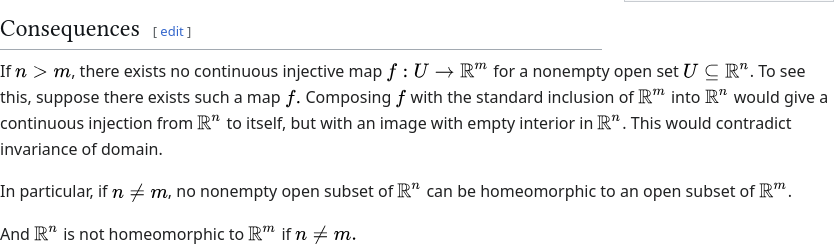
\includegraphics[width=0.75\linewidth]{img mono/schoenflies/inv dominio.png}
    	\caption{agregar esto}
\end{figure}

% Podemos usar la invariancia del dominio para probar lo siguiente:

\begin{lema}\label{puntos separan}
    Sea $M$ una $n$-variedad conexa con $n<1$, $P\subset M$ un conjunto finito, entonces $M-P$ es conexo.
\end{lema}

% \comm{esta prueba es de las notas de Nikil Sahoo}

\begin{proof}
    Primero comenzamos observando que como nuestros espacios son Hausdorff, entonces los singleton $\{p\}$ son conjuntos cerrados. Por esta razón, los complementos de finitos puntos son subconjuntos abiertos de $M$, y por lo tanto son $n$-variedades.

    Por lo tanto, es suficiente probar el lema para $P=\{p\}$ un singleton. Veamos eso.

    Supongamos por absurdo que $M-\{p\}$ no es conexo, es decir, tenemos $U, V$ dos abiertos de $M-\{p\}$ tales que $M-\{p\}=U\sqcup V$. Estos también van a ser abiertos de $M$.

    \duda{por que son abiertos de M necesariamente?}

    Tomamos un entorno $U_p$ de $p$ en $M$ homeomorfo a $\D^n$, entonces $U_p - \{p\}$ es conexo, y por lo tanto está contenido en $U$ o en $V$. Supongamos que está en $U$, en ese caso $U_p-\{p\}\subset U$, y $U_p\cup U = U\cup\{p\}$, como ambos $U_p$ y $U$ son abiertos de $M$. Entonces $U\cup \{p\}$ es abierto en $M$ y obtenemos una descomposición de $M$ como dos abiertos disjuntos $(U\cup\{p\})\sqcup V$. Esto es absurdo ya que habíamos asumido $M$ conexa.
\end{proof}

\begin{teo}
    Teo 1.8.3: Dada $\Sigma$ una $(n-1)$-esfera encajada en $\s^n$, sea $G$ uno de los dominios complementarios. Entonces, si $\overline{G}$ es una variedad, necesariamente es una $n$-bola.
\end{teo}

\begin{proof}
Como es una variedad, entonces $\Sigma$ tiene entornos de collar locales. Por el teorema de Schoenflies generalizado entonces es una $n$-bola.
\end{proof}

% \comm{leer https://mathoverflow.net/questions/29737/understand-cech-cohomology}


% \section{truco de Klee}

\begin{teo}
    Extensión de Tietze: Sea $X$ un espacio topológico normal y $C\subset X$ un cerrado. 
    Entonces, cualquier función continua $f:C\to [0,1]$ se extiende a una función continua de dominio $X$.
\end{teo}

\begin{obs}
    Esto vale en general para productos de $[0,1]$, podemos observar eso viendo $f\colon C\to[0,1]^k$ como funciones coordenadas $f_i\colon C\to [0,1]$ para $i\in\{1,\dots,k\}$.
\end{obs}

\comm{definir normal}

\begin{teo}
    2.5.1 Klee trick: Sea $D$ una $k$-bola encajada en $\R^{n}$. Entonces, el encaje obtenido componiendo con la inclusión $\R^n\hookrightarrow \R^{n+k}$ es plano en $\R^{n+k}$.
\end{teo}

\begin{proof} (Rushing)

    $D$ es una $k$-bola, entonces tenemos un homeo $h_*\colon D\to \D \subset\R^k$. Por el teorema de extensión de Tietze, puedo extender este homeo a una función continua $\tilde{h}\colon\R^{k}\to [0,1]^k$.

    Consideramos la función $\phi_f\colon \R^{n+k}\to \R^{n+k}$ dada por $\phi_f(x,y):=\left(x,y+f(x)\right)$ para $x\in\R^n$, $y\in\R^k$. Observar que esta función "preserva" los planos $\{r\}\times\R^k$

    Si tomamos un punto $x\in D\subset \R^n$, al pasar por la inclusión podemos verlo como $(x,0)\in\R^{n+k}$. Aplicando $\phi_f$ a $(x,0)$ obtenemos $(x, f(x))$.

    Como $f\colon D\to[0,1]^k$ es un homeo, en particular es inyectiva, y con esto tenemos que $\phi_f$ es inyectiva en $D\times\{0\}$.

\end{proof} 

\begin{teo}(Davenma y Venema)

    Sea $C$ un espacio compacto $T_1$, y sean $\lambda\colon C\to\R^n$ y $\lambda'\colon C\to R^m$ encajes. Entonces, los encajes $e, e'\colon C\to R^n\times\R^m$ dados por $e(c):=\left(\lambda(c),0\right)$ y $e'(c):=\left(0, \lambda'(c)\right)$ son equivalentes al encaje diagonal $d=\lambda\times\lambda'\colon C\to \R^n\times\R^m$.

\end{teo}

\begin{proof}

Veamos que $e$ es equivalente a $d$, luego para $e'$ es un razonamiento análogo.

Primero, observamos que por el teorema de extensión de Tietze podemos extender $\lambda'\circ\lambda^{-1}\colon \lambda(C)\to \R^m$ a una función continua $\psi\colon \R^n\to\R^m$. 

Definimos $\Psi\colon\R^n\times\R^m\to\R^n\times\R^m$ dada por $\Psi(x,y)=\left(x,y+\psi(x)\right)$. Entonces, $\Psi$ es continua y además es un homeomorfismo, ya que su inversa está dada por $\Psi^{-1}(x,y)=\left(x,y-\psi(x)\right)$, que también es continua.

Luego, $\Psi$ cumple $$\Psi\circ e(c)=\Psi\left(\lambda(c),0\right)=\left(\lambda(c),\psi\circ \lambda(c)\right)=\left(\lambda(c),\lambda'(c)\right)=d(c)$$ y con eso tenemos la equivalencia buscada.

\end{proof}

% \chapter{Planaridad local}

Platera de cosas para probar:

Teo 3.6.1: Taming theorem

Cor 3.6.1: Condiciones para que un encaje localmente plano entre PLs sea $\epsilon (x)$-tame manteniendo fijo un poliedro.

Teo 3.3.3: Dada $\Sigma\subset\s^n$ una $(n-1)$-esfera con $n\geq 4$ tal que $\Sigma -\{p\}$ es localmente plana en $\s^n$ y $\Sigma$ tiene entornos de collar locales en $p$ para uno de los dominios complementarios de $\s^n-\Sigma$. Entonces, $\Sigma$ es plana. 

Teo 3.3.2: Dada $\Sigma\subset\s^n$ una $(n-1)$-esfera con $n\geq 4$, $p\in\Sigma$ tal que $\Sigma - \{p\}$ tiene entornos de collar locales en uno de los dominios complementarios, entonces la clausura de ese dominio es una $n$-bola.

Lema 3.3.1: tecnico

Teo 3.2.1: Dado un arco $\alpha\subset\R^n,\, n\geq 4$ que es localmente poliedral salvo en un conjunto numerable $X\subset\alpha$, entonces, $\alpha$ es plano en $\R^n$.

Teo 1.8.3: Dada $\Sigma\subset\s^n$ una $(n-1)$-esfera, y sea $D$ uno de los dominios complementarios. Si $\overline{D}$ es una variedad, entonces es una $n$-bola.
Dem: Ejercicio.

Ej 1.8.4: Una función $f\colon\s^{n-1}\to\s^n$ es plana si y solo si la clausura de sus dominios complementarios son $n$-bolas.

Teo 1.7.3: Una subvariedad tiene entornos de collar locales, entonces tiene entorno de collar global.

Ej 1.7.3: El borde de una variedad siempre tiene entorno de collar local.

Teo 1.7.4: El borde de una variedad con borde tiene entorno de collar.

Teo 1.7.5: M conexa, sin borde, localmente plana, two-sided, $(n-1)$-submanifold de una $n$-variedad $N$. Entonces, $M$ tiene entorno de bicollar en $N$.

Teo 1.7.6: Pinched bicollar thm:\begin{itemize}
	\item Dado un cerrado $X\subset M\subset N$, si $M-X$ tiene entornos de collar locales en $N$, entonces $M$ tiene un collar pinchado en $X$.
	\item Dado un cerrado $X\subset M$, existe un collar de $\partial M$ en $M$ pinchado en $X$.
	\item Dada $M\subset N$ subvariedad de codimensión 1, $X\subset M$ cerrado, si $M-X$ es una subvariedad two sided, conexa, localmente plana del interior de $N$, entonces existe un bicollar de $M$ en $N$ pinchado en $X$.
\end{itemize}
Dem: Ejercicio (1.7.10)







\comm{davenma y venema}

\begin{df}
Dados dos cerrados $A$, $B$ de un espacio $X$, consideramos en $A\times[0,1]$ la relación de equivalencia cuyas clases no triviales están dadas por $$(x,t)\sim (x,t')\iff x\in A\cap B$$
Llamamos \textbf{collar de A pinchado en B} a un encaje $h\colon A\times[0,1]/_{\sim}\to X$ tal que \begin{itemize}
\item $h(x,0)=x$ para todo $x\in A$
\item $h(A\times [0,1]/_\sim)$ es un entorno de $A - B$
\end{itemize}
\end{df} \duda{buscar una mejor traducción, en realidad es pinched collar}

\begin{lema}
	Sean $A$, $B$ cerrados de $X$ tal que $A$ tiene entornos de collar locales en $X$ para todo punto de $A-B$. Entonces, existe un collar de $A$ pinchado en $B$.
\end{lema}

\begin{lema}
	Sea $h\colon\Delta^n\to \s^n$, con $n\geq 4$, un encaje de un $n$-símplice en $\s^n$ tal que es lineal a trozos en todo $\Delta^n$ salvo un vértice. Entonces, $\s^n - \mathring{(\Delta^n)}$ es una $n$-bola.
\end{lema}

\begin{proof}
Sea $h\colon\Delta^n\to\s^n$ un encaje que es lineal a trozos en $\Delta^n - \{v\}$ para $v$ un vértice de $\Delta^n$. 

Tomamos $A$ un $n$-símplice tal que $\Delta^n\subset A$ y $\partial A\cap\Delta^n=\{v\}$ como en la imagen \ref{simp1}.

Sea $B$ un $n$-símplice contenido en el interior de $\Delta^n$. Dado un vértice $w\in B$, consideramos $\alpha$ el segmento lineal que va de $v$ a $w$. Como los símplices son convexos, a menos de algunos ajustes podemos asegurarnos que $\alpha\cap B=\{w\}$, como en la imagen \ref{simp2}.

Como el encaje $h$ es lineal a trozos en todo $\Delta^n$ salvo $\{v\}$, sabemos que $h|_{\Delta^n - \{v\}}$ se extiende a un encaje lineal a trozos $\hat{h}$ de $\left(\Delta^n - \{v\}\right)\times [0,1]$, es decir, se extiende a un entorno collar de $\Delta^n - \{v\}$. Por el lema anterior entonces podemos decir que $\Delta^n$ tiene un entorno de collar pinchado en $\{v\}$. Convenientemente este entorno es como en la imagen \ref{simp1}, lo que nos dice que podemos ver $\hat{h}$ como un encaje topológico (no PL) de $A$ en $\s^n$. 

Por el lema anterior, el encaje $h$ 
\end{proof}

\begin{figure}
    	\centering
    	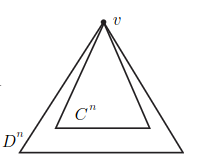
\includegraphics[width=0.35\linewidth]{img mono/casi plano/1.png}
    	\caption{Dibujito}
        \label{simp1}
\end{figure}

\begin{figure}
    	\centering
    	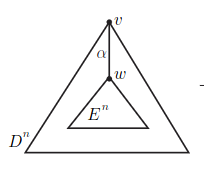
\includegraphics[width=0.35\linewidth]{img mono/casi plano/2.png}
    	\caption{Dibujito}
        \label{simp2}
\end{figure}



\comm{kirby}

Sea $C$ un subconjunto no vacío de un Cantor ternario estándar en $[-1,1]$. Supongamos que $\{-1,\,1\}\in C$. Tomamos $D:=\{d_1,d_2\dots\}$ un subconjunto numerable y denso en $[-1,1]\cap C^c$ (por ejemplo, tomar los puntos medios de los intervalos que se van eliminando para definir $C$).

Consideramos la siguiente curva $J$ en $\s^{n-1}$:
$$J:=\left\{(x_1,\dots, x_n)\in\s^n\subset\R^n\colon x_{n-1}^2+ x_{n}^2=1,\, x_{n-1}\geq 0, x_1=x_2=\dots = x_{n-2}=0\right\}$$

\begin{figure}
    	\centering
    	\includegraphics[width=0.4\linewidth]{img mono/kirby/j.png}
    	\caption{La curva $J$ en $\s^2$}
        \label{jota}
\end{figure}

Identificamos $[-1,1]$ con la 

% \chapter{misc}

\comm{definir poliedral: lineal a trozos con finitos trozos}

\begin{teo}
Sea $\alpha\subset\R^n$, con $n\geq 4$ un arco localmente poliedral salvo un conjunto numerable $X\subset \alpha$. Entonces, $\alpha$ es plana en $\R^n$.
\end{teo}
\begin{proof}
\comm{falta justificar pq el arco estaría compuesto x numerables segmentos}
Extendiendo cada segmento de $\alpha$ obtenemos una familia de recta. Agregamos a esta familia una recta que pase por cada punto de $X$, llamamos $\{r_i\}$ a la familia. Cada par de estas rectas determina un plano $H_{ij}$ de dimensión
\end{proof}

\begin{teo}
Teo 3.3.1 Cantrell: Sea $\Sigma$ una $(n-1)$-esfera en $\s^n$ con $n\geq 4$, $p\in\Sigma$ un punto tal que $\Sigma$ es localmente plana en todo punto de $\Sigma -\{p\}$. Entonces, $\Sigma$ es plana en $\s^n$.
\end{teo}

\begin{teo}
Teo 3.3.2 Cantrell: Sea $\Sigma$ una $(n-1)$-esfera en $\s^n$ con $n\geq 4$, $p\in\Sigma$ un punto, $D\subset \s^n - \Sigma$ una de las componentes conexas del complemento. Entonces, si $\Sigma -\{p\}$ tiene entornos de collar locales en $\overline{D}$, se cumple que $\overline{D}$ es una $n$-bola. 
\end{teo}

\begin{proof}
$\Sigma$ es un $(n-1)$-esfera, por lo tanto podemos considerar un homeo $h\colon\partial B(0,1)\to \Sigma$, al que además le pedimos que $h\left((0,\dots,0,1)\right)=p$.

Definimos $C_t:=\{(x_1,\dots,x_n)\in\R^n \,|\, x_1^2+x_2^2+\dots+x_{n-1}^2+(x_n + t)^2 \leq (1-t)^2 \}$
\comm{imagen}

Como $\Sigma - \{p\}$ tiene entornos de collar locales en $\overline{D}$, el homeo $h$ puede extenderse a un encaje $g\colon\overline{C_1-B\left(0,1\right)}\to\overline{D}$, cuyo dominio es un entorno de collar de $B(0,1)$ pinchado en $h^{-1}(p)$ como en la imagen \ref{3}. \comm{escribir bien esto}

\begin{figure}
    	\centering
    	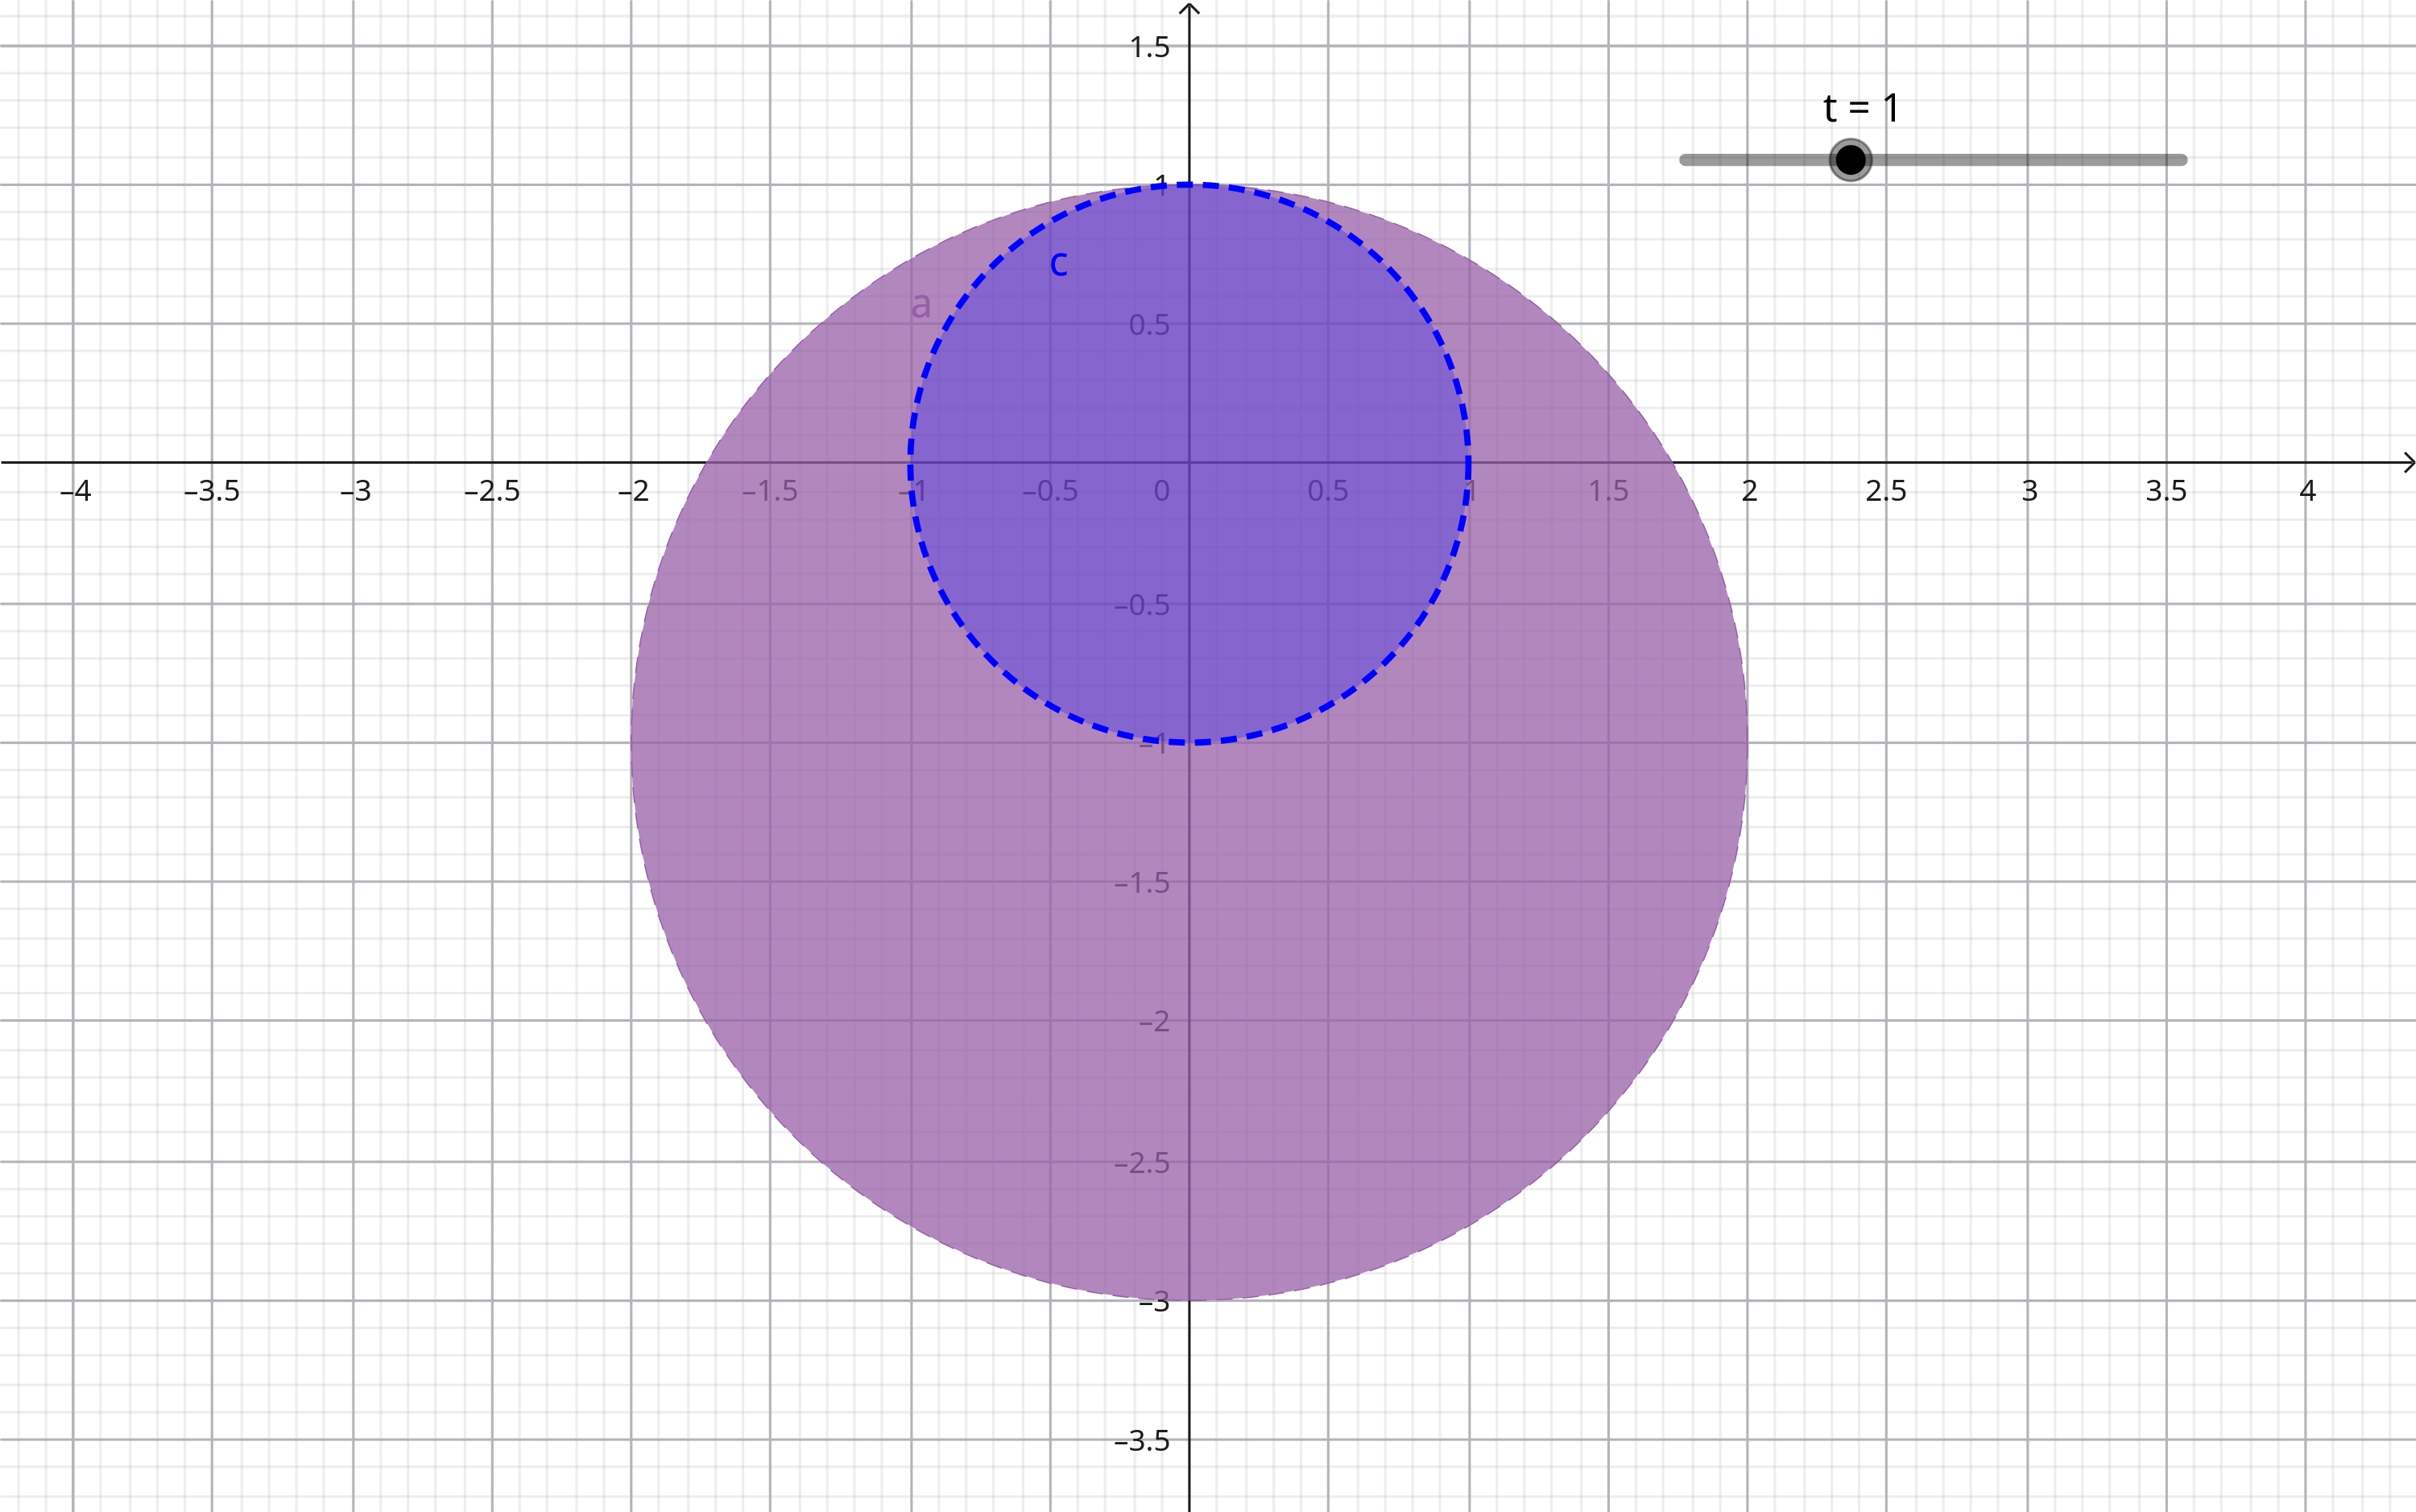
\includegraphics[width=0.55\linewidth]{img mono/casi plano/3.png}
    	\caption{Dibujito}
        \label{3}
\end{figure}

Llamamos: \begin{itemize}
\item $R_1$ la componente conexa de $\s^n - g(\partial C_\frac{1}{2})$ que está contenida en $D$
\item $R_2$ la componente conexa de $\s^n - g(\partial C_1)$ que está contenida en $D$
\end{itemize}\comm{dibujos}

Observación: $\overline{\R_1}\cong \overline{D}$.

Sea $h_*:\R^n\to\R^n$ un homeo que manda $\partial C_\frac{1}{2}$ en $\partial B(0,1)$ y tal que deja fijo $\partial C_1$. 

Consideramos la función $$f(x)=\begin{cases}
x,\quad x\in R_2\\
gh_*g^{-1}(x),\quad x\in\overline{R_1-R_2}
\end{cases}$$
Entonces, $f$ es un homeo que manda $\overline{R_1}$ en $\overline{D}$.

Por lo tanto, obtenemos lo siguiente: Si pegamos una copia de $\overline{R_1}$ a $\overline{C_\frac{1}{2}-B(0,1)}$ por $\partial C_\frac{1}{2}$ mediante $g^{-1}|_{g(\partial C_\frac{1}{2})}$, como $g$ es un homeo en $\overline{C_1-B(0,1)}$ y estamos "cambiando" un espacio por otro que es homeomorfo al original, entonces el nuevo espacio obtenido es homeo a $\overline{R_1}$, es decir, homeomorfo a $\overline{D}$. Vamos a usar esto para probar que $\overline{R_1}$ es una $n$-bola, y por lo tanto que $\overline{D}$ también lo es.\comm{dibujo}

Sea $S$ una $(n-1)$-esfera encajada de forma plana en $\overline{C_\frac{1}{2}-B(0,1)}$ tal que $$S\cap \left(\partial C_\frac{1}{2}\cup\partial B(0,1)\right)=(0,\dots,0,1)$$ 

Sea $K$ la componente conexa de $\s^n-g(S)$ que contiene a $R_1$. \comm{dibujo}

Por el teorema 3.3.3, tenemos que $\overline{K}$ es una $n$-bola.\duda{por qué tiene entorno de collar en $p$? el teo 3.3.3 requiere esto. supongo que si porque la región $\overline{C_\frac{1}{2}-B(0,1)}$ eeee. justificar.mas q nada la pregunta sería por qué la puedo encajar de forma plana}

Llamamos $\text{Int}(S)$ a la componente conexa de $\R^n - S$ que no intersecta a $g^{-1}(\Sigma)=\partial B(0,1)$. 

Sea $P:=\overline{C_\frac{1}{2}-B(0,1)}-\text{Int}(S)$. Consideramos $P'$ el pegado de P con $\overline{D'}$ (la otra cc además de $D$) por $\partial B(0,1)$ mediante $g^{-1}|_\Sigma$. Luego consideramos $P''$ el pegado de $P'$ con $\overline{R_1}$ por $\partial C_\frac{1}{2}$ mediante $g^{-1}|_{\partial R_1}$. Observamos que el espacio obtenido $P''$ es una $n$-bola. \comm{dibujo, poner el $P$ para mostrar que tiene dos agujeros.}

% Entonces, $P''$ es una $n$-bola (la clausura del exterior de $S$)

Dada una bola estándar en $\R^n$ centrada en $(0,\dots,0,1,0)$ y de radio $1$, notamos $F$ a los puntos $(x_1,\dots,x_n)$ de la bola que cumplen $x_n\geq 0$. Consideramos una sucesión $\{q_i\}_{i=0}^\infty$ contenida en la intersección de $\partial F$ con el plano dado por $x_i=0$ para todo $i\in\{1,\dots,n-2\}$. Definimos $\{q_i\}$ como una sucesión que cumpla lo siguiente:\begin{itemize}
\item Si $q_i=(0,\dots,0,a_{(n-1)}^i, a_n^i)$, entonces $a_{(n-1)}^0 = 2$ y $a_{n}^0=0$ (empiezan en el punto (0,0,...,2,0))
\item Los $a_{n-1}^i$ convergen a $0$ monótonamente. (la penúltima coordenada decrece monótonamente a $0$, como en la imagen)
\item $a_n^i > 0$ si $i>0$. (van por la curva de arriba, la cáscara de la bola, no por el plano)
\end{itemize}\comm{imagen}

Usamos estos puntos para trazar planos y delimitar una partición del conjunto $F$. Consideramos el plano de dimensión $(n-2)$ dado por $x_{n-1}=x_n=0$. Dado $i\in\N$, consideramos la suma (directa) de la recta que pasa por $0$ y $q_i$ con este plano. Como el $(n-2)$-plano intersecta al otro plano que usamos para definir la sucesión de los $q_i$ sólamente en el $0$, entonces están en suma directa. Esto implica que el espacio obtenido al sumar el $(n-2)$-plano con la recta que pasa por $0$ y $q_i$ es un $(n-1)$-plano.

Para hacer una analogía en dimensión $3$, nuestro $n-2$ plano simplemente sería la recta del eje $x$. Al sumar esta recta a un $q_i$, obtenemos un plano (de dimensión $2$) que pasa por $q_i$ y contiene la recta del eje $x$. La idea es considerar uno de estos planos pasando por cada $q_i$, y esto va a delimitar una partición (en este caso de la bola de centro $(0,1,0)$ y radio $1$) del conjunto $F$ en "gajos", que son el espacio entremedio de dos planos adyacentes. \comm{dibujo}

Llamamos $D_i$ a las regiones en $F$ delimitadas entre los $(n-1)$-planos que pasan por $q_{i-1}$ y $q_i$. Como son regiones entre planos intersectadas con una (media) $n$-bola, entonces son $n$-bolas.

Consideramos $D_i'$ una $n$-bola (y similar a $D_i$ en forma, o sea nada muy loco xd), tal que $D_i'$ está contenida en $D_i$ salvo por el punto $(0,\dots,0)$. 

Observamos que al unir dos copias consecutivas $(D_i - \mathring{D_i'})$ y $(D_{i+1} - \mathring{D}_{i+1}')$ obtenemos un espacio homeomorfo a $P$. En referencia a esto llamamos \begin{align*}
& P_i:=(D_{2i-1} - \mathring{D}_{2i-1}') \cup (D_{2i} - \mathring{D}_{2i}') \quad \text{si } i\text{ es par } \\
& P_i':=(D_{2i} - \mathring{D}_{2i}') \cup (D_{2i+1} - \mathring{D}_{2i+1}') \quad \text{si } i\text{ es impar }
\end{align*}\comm{dibujo}

Observar que los $P_i$ y $P_i'$ comparten $D_{2i}-\mathring{D_{2i}'}$, y los $P_i'$ y $P_{i+1}$ comparten $D_{2i+1}-\mathring{D_{2i+1}'}$.

Llamamos $\omega_i$ a $\partial D_i'$. Definimos homeomorfismos $$\phi_i\colon P_i\to P_i',\quad \psi_i\colon P_i'\to P_{i+1}$$
tales que \begin{align*}
	& \phi_i(\omega_{2i-1})=\omega_{2i+1},\quad\phi_i|_{\omega_{2i}}=\text{Id}\\
	& \psi_i(\omega_{2i})=\omega_{2i+2},\quad\psi_i|_{\omega_{2i+1}}=\text{Id}
\end{align*}
para poder cumplir estas condiciones, es necesario pedir $n\geq 3$. (en ese caso podemos "fluir" alrededor de la esfera $\omega_k$ que quedaría fija)

Identificamos la terna $(P_1,\omega_1,\omega_2)$ con $(P,\partial C_{\frac{1}{2}},\partial B_1)$. Luego identificamos $\omega_1$ con $\partial R_1$ y $\omega_2$ con $\partial D'=\Sigma$, mediante $g$. De igual manera que antes, obtenemos una $n$-bola a la que llamaremos $\tilde{P_1}$.

De forma similar vamos a definir pegados para el resto de los $P_i$ y $P_i'$, componiendo el homeo $g$ con los $\phi_i$ y $\phi_i$. Lo que hacemos es pegar el borde de $R_1$ y $D'$ a $\omega_{2i+1}$ y $\omega_{2i+2}$ respectivamente, mediante los homeomorfismos\begin{align*}
	& \phi_i\circ\dots\circ\phi_2\circ\phi_1\circ g^{-1}\colon\partial R_1\to\omega_{2i+1}\\
	& \psi_i\circ\dots\circ\phi_2\circ\phi_1\circ g^{-1}\colon\partial D'\to\omega_{2i+2}
\end{align*}
De igual forma los conjuntos obtenidos son $n$-bolas, y los notamos $\tilde{P}_i$ y $\tilde{P}_i'$.

Como $\phi_1$ es la identidad en $\omega_2$, podemos extenderla a un homeo $\tilde{\phi}_i\colon\tilde{P}_1\to\tilde{P}_1'$, y por lo tanto $\tilde{P}_1'$ es una $n$-bola. De la misma forma podemos hacer esto con cada $\phi_i$ y $\psi_i$, y obtener que todos los $\tilde{P}_i$ y $\tilde{P}_i'$ son $n$-bolas.

Definimos $F_1:=\cup_{i=1}^\infty\tilde{P}_i$, luego $F_1$ es una $n$-bola.\comm{no me convence, justificar}

Observamos que $\partial(D_{2i-1}\cup D_{2i}) = \partial\tilde{P}_i$. Como $D_{2i-1}\cup D_{2i}$ y $\tilde{P}_i$ son $n$-bolas, el homeomorfismo entre sus bordes dado por la identidad se extiende a un homeomorfismo entre $D_{2i-1}\cup D_{2i}$ y $\tilde{P}_i$.\comm{no entiendo el punto de esto, como ya sé que son $n$-bolas no tengo siempre el homeomorfismo? mm capaz para asegurar q sea Id en el borde}

Tomando estas extensiones para todo $i$ obtenemos un homeo de $F$ en $F_1$. \comm{de nuevo no me convence, justificar. entiendo que la sucesión que es ir sumando de a un homeo converge, escribir bien}

Observamos que $F_1$

Consideramos $\tilde{P}_1$ contenido en $F_1$, y eliminamos de $\tilde{P}_1$ el interior de la $n$-bola $R_1$ que le habíamos pegado. 

\end{proof}


\begin{teo}
Teo 3.3.3: Sea $\Sigma$ una $(n-1)$-esfera en $\s^n$ con $n\geq 4$, $p\in\Sigma$ un punto. Sean $D\subset \s^n - \Sigma$ una de las componentes conexas del complemento. Si $\Sigma$ es localmente plana en $\s^n$ y $\Sigma$ tiene entornos de collar locales en $\overline{D}$, entonces $\Sigma$ es plana en $\s^n$.
\end{teo}

\begin{teo}
Teo 1.8.3: Lo voy a pasar a la parte de Schoenflies
\end{teo}

\begin{proof}
Tenemos una $(n-1)$-esfera $\Sigma$ encajada en $\s^n$, $p$ un punto de $\Sigma$, $G$ y $H$ las componentes conexas de $\s^n - \Sigma$. Suponemos que $\Sigma$ está encajada de forma localmente plana en $\S^n$ y $\Sigma$ tiene entornos de collar locales para $p$ en $\overline{H}$. Entonces, $\Sigma$ es plana.

Como $\Sigma$ tiene entornos de collar locales en $\overline{H}$, por el teorema de Schoenflies generalizado es una $n$-bola.
\comm{chequear esto y citar bien}
\end{proof}

\begin{lema}
Lema 3.3.1: Sea $\Sigma$ una $(n-1)$-esfera en $\s^n$, $p\in\Sigma$ un punto, $D$ y $D'$ las componentes conexas de $\s^n - \Sigma$. Supongamos que $\Sigma-\{p\}$ es localmente plana en $\s^n$, $\Sigma$ tiene entornos de collar locales en $\overline{D}$, y existe un homeo $h\colon\partial B(0,1)\to\Sigma$ tal que $h\left((0,\dots,0,1)\right)=p$.

Entonces, $h$ puede extenderse a un encaje $g\colon\overline{C_1-B\left(0,\frac{1}{4}\right)}\to\s^n$.
\end{lema}

\begin{proof}
Sale por los entornos de collar.
\end{proof}

% \chapter{Un ejemplo de Fox y Artin}

\lipsum[3]

% \chapter{Un ejemplo de R H Bing}

Ejemplo: Una 2-esfera salvaje $S$ y una curva cerrada simple $J\subset\R^3-S$ tales que 
\begin{itemize}
    \item $J$ no es trivial en $\R^3-S$
    \item Para todo disco $D\subset S$, $J$ es trivial en $\R^3-D$
\end{itemize}
              
Partimos de $S_0$ una esfera domesticada. 

Sea $E_1,\dots,E_n$ una descomposición celular de $S_0$ \comm{definir} tal que $E_i$ y $E_{i+1}$ comparten borde para todo $i\in\{1,\dots,n-1\}$, y $E_1$, $E_n$ también compartan borde. 

Engordamos las células $E_i$ \duda{¿qué debería decir? tomar entorno tubular? tendría que definir mejor esto} y les agregamos un cilindro con un asa al final $H_i$ para obtener un toro $T_i$, de manera que el agujero de $T_i$ encierre al cilindro de $H_{i+1}$. De la misma manera $H_n$ encierra el cilindro de $H_1$. 
            
Consideramos $H_i$ toros sólidos, a los que nos referiremos como "lazos", y tomamos $E_i'$ un entorno tubular de $E_i$. 
            
Definimos $T_i$ como el pegado de $E_i'$ con $H_i$ por un disco, de manera que el agujero de $H_i$ encierre a $T_{i+1}$ como se ve en la imagen. 

Más específicamente, consideramos una 2-célula $C_i$ y pegamos $\partial C_i$ con $\gamma_i\subset T_i$ una curva no contractible en $T_i$, llamamos a este pegado $T_i'$. 
            
Ahora colapsamos $C_i$, es decir, cocientamos $T_i'$ por la relación $x\sim y \Leftrightarrow x,y\in C_i$. Definimos el pegado de arriba de manera que, al hacer este colapso, el cociente de $T_{i+1}$ tenga dos componentes conexas: una que contiene a $E_{i+1}'$ y otra que es un toro.

Llamamos $W_1=\bigcup\limits_{i=1}^n T_i$. 

La 2-esfera $S$ del ejemplo va a estar contenida en $W_1$, y va a intersectar a $\bigcup\limits_{i=1}^n\partial T_i$ sólamente en $\bigcup\limits_{i=1}^n\partial E_i$.

\begin{figure}[h!]
    \centering
    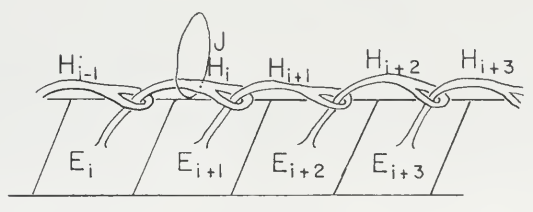
\includegraphics[width=0.5\linewidth]{img mono/hooked rug/1.png}
    \caption{$J$ no trivial en $W_i$}
    \label{hr1}
\end{figure}
            
Por el teo 11 una curva $J$ como en la imagen es no trivial en $\R^3-W_1$ \comm{justificar mejor} 

Ahora sacamos un cilindro sólido de cada $H_i$ para obtener un cubo topológico $K_i$. \duda{cubo topológico? por qué no decir esfera sólida/bola? yo le copié al bing}

Observar que $\partial E_i$ divide $\partial K_i$ en dos discos, uno que está contenido en la componente acotada de $\R^3-S_0$ y otro que está contenido en $H_i$ pero que ya no encierra a $H_{i+1}$. 
            
Llamamos a este segundo disco $D_i$.  
          
Movemos homotópicamente el interior de este segundo disco de manera que quede contenido en $int(T_i)$. Entonces tenemos $D_i\subset int(T_i)$ y $\partial D_i=\partial E_i$. 

Luego $\bigcup\limits_{i=1}^n D_i$ es una esfera, a la que llamamos $S_1$. 

Ahora subdividimos cada $D_i$ en 2-células $E^i_1,\dots, E^i_{15}$ tal que $E^{i}_{j},E^{i}_{j+1}$ comparten borde para todo $i\in\{1,\dots,14\}$, $E^{i}_{15}$ y $E^{i}_{1}$ compartan borde. \duda{q pasa si usamos otros números? obtenemos esferas no equivalentes supongo. y qué pasa si usamos x ejemplo n=2? funciona igual?} 

Continuamos con un proceso similar. Ahora engordamos los $E^i_j$ y les pegamos un toro $H_i$ por un disco para formar un toro sólido $T^i_j$, que de la misma manera que antes encierra a $T^i_{j+1}$ para todo $j\in\{1,\dots, 14\}$, y $T^i_{15}$ encierra a $T^i_1$.  
            
Además pedimos que dos cilindros de $T^i_j$ no consecutivos, por ejemplo $T^i_7$ y $T^i_{11}$, se enrieden como en la siguiente imagen: \duda{no me queda claro si pedir q no sean consecutivos es lo único que se necesita}

\begin{figure}[h!]
    \centering
    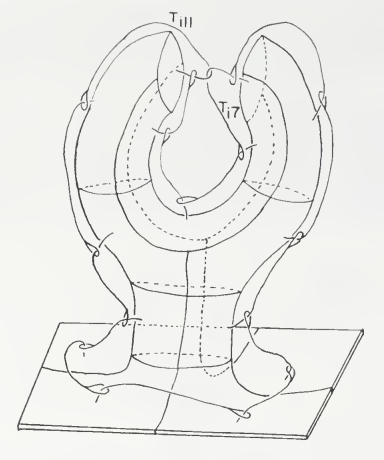
\includegraphics[width=0.5\linewidth]{img mono/hooked rug/2.png}
    \caption{$T^i_j$ se enriedan}
    \label{hr2}
\end{figure}

Por los teoremas 9 y 11 tenemos que cualquier curva cerrada no trivial en $\R^3 - T_i$ es no trivial en $\R^3-\sum T^i_j$. \comm{justificar}
            
Hacemos esta construcción de manera que $\bigcup\limits_{j=1}^{15} T^i_j\subset T^i$, es decir, tomamos los $T^i_j$ bien pegaditos a los $E^i_j$. (También puedo decir que están bien pegaditos al $D_i$) 

De la misma forma que antes, sacamos un cilindro sólido de cada $T^i_j$ para obtener un cubo $K^i_j$, cuyo borde es separado en dos discos por $\partial E^i_j$. Llamamos $D^i_j$ al disco contenido en la componente conexa de $T^i_j-E^i_J$ que es un toro, y movemos $int(D_j^i)$ mediante una homotopía para que quede contenido en $int(T_j^i)$. 

Llamamos entonces $S_2$ a la esfera $\bigcup\limits_{i,j} D^i_j$. También llamamos $W_2$ a $\bigcup\limits_{i,j}T^i_j$ 

El ejemplo $S$ es el límite de la secuencia $\{S_i\}_{i\in\N}$, y también es $S=\bigcap\limits_{i\in\N}W_i$, con $W_i$ 3-variedades con borde. \duda{ustificar por qué la secuencia tiene límite y cómo defino eso y tb justificar por qué la intersección de los $W_i$ es una variedad sin borde.}

En general, para obtener $S_{n+1}$ y $W_{n+1}$ a partir de $S_n=\bigcup\limits_{i=1}^{15}D_i$ y $W_n=\bigcup\limits_{i=1}^{15}T_i$ el proceso es el siguiente: 
            
Subdividimos cada disco $D_i$ de la construcción de $S_n$ en 15 discos que llamaremos $E^i_1,\dots, E^i_{15}$, luego tomamos sus entornos tubulares $E^{i'}_{j}$ y los pegamos con un toro $H_j^i$ por un disco, obteniendo toros $T^i_1,\dots,T^i_{15}$ de manera que queden enganchados como describimos antes, y de manera que dos lazos $T_j^i$ y $T_k^i$ no consecutivos se enrieden entre sí como se mostraba en la imagen. 
            
Además nos aseguramos de tomar estos $T_j^i$ bien cerca de $D_i$ para que $\bigcup\limits_{j} T^i_j\subset T_i$

La 3-variedad con borde $W_{n+1}$ la definimos como $\bigcup\limits_{i,j} T_j^i$ y cumple $W_{n+1}\subset W_n$. 

Después sacamos un cilindro de cada uno de los toros $T_j^i$ para obtener cubos $K_j^i$, que son separados por $\partial E_j^i$ en dos discos. 

Llamamos $D_j^i$ al disco contenido en la componente conexa de $T_j^i - E_j^i$ que es un toro, y movemos $int(D_j^i)$ mediante una homotopía para que quede contenido en $int(T_j^i)$. 

Definimos $S_{n+1} = \bigcup\limits_{i,j} D_j^i$. 

¿Por qué este límite es una esfera?

Sea $S_n=\bigcup D_i$ como en la construcción, entonces $\partial D_i\subset S_{n+k} \fall k\in\N \Rightarrow \partial D_i\subset \lim\limits_{n\to\infty} S_n$ 

Además, dados $D_{i_1},D_{i_2}$ discos de la construcción de $S_n$, se tiene que $D_{i_1}\cap D_{i_2}=\varnothing$ y como $D_i\subset W_n$ y sus subsecuentes modificaciones van a seguir estando en $W_{n+k}$ y por lo tanto las modificaciones no se van a intersectar. \duda{r h what are you trying to tell me} 

\begin{figure}[h!]
    \centering
    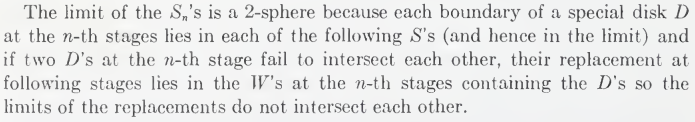
\includegraphics[width=0.5\linewidth]{img mono/hooked rug/esfera.png}
    \caption{tengo que escribir bien esto}
    \label{esfera}
\end{figure}

Entre cada $S_n, S_{n+1}$ tenemos un homeo $h_n$ \comm{escribirlo explícitamente}

Si definimos estos homeos para que $\{f_n=h_n\circ\dots\circ h_0\}_{n\in\N}$ converjan uniformemente, entonces existe el límite $f:S_0\to S$ y es continua. 

Si $f$ fuera biyectiva entonces sería un homeo porque $S_0$ compacto y $S$ es Hausdorff \comm{poner prueba de esto y de por qué S es hff}
 

$\textbf{Afirmación:}$ Si $J$ es una curva cerrada simple como en la primer imagen, entonces $J$ no es homotópica a un punto en $\R^3 - S$ 

\begin{dem}
          
$J\sim\ast$ en $\s^c \Rightarrow J\sim\ast$ en $(\bigcap\limits_{i\in\N} W_i)^c\Rightarrow J\sim\ast$ en $\bigcup\limits_{i\in\N} W_i^c\Rightarrow J\sim\ast$ en algún $W_i^c$

Veamos que tener una homotopía de $J$ a un punto en algún $W_i^c$ es absurdo. 

Sea $W_i'$ el conjunto obtenido rellenando los agujeros de $W_i$ \duda{me parece raro decir esto así}, entonces $W_i'$ es una esfera \comm{o una "bola hueca" porque en realidad estamos tomando un entorno tubular del borde, pero no sé si importa decir esto} con manijas y sea $W_i''$ el conjunto obtenido quitando un cilindro de cada agujero en $W_i$ \duda{también esto xd y no entendí lo que sigue} \end{dem}

\begin{teo}{Teorema 9} Sea $C$ un cilindro con bases $B_1$ y $B_2$, sean $T_1,\; T_2$ dos toros enganchados entre sí \duda{se puede decir así esto?} tales que $T_i\cap\partial C=B_i$ y sea $X\subset\R^3$ un cerrado tal que $X\cap C=B_1\cup B_2$. 
          
Entonces, dada una curva simple y cerrada $J \subset (X\cup C)^c$, tenemos que $J$ no es homotópica a un punto en $(X\cup T_1\cup T_2)^c$ \end{teo}

\begin{figure}[h!]
    \centering
    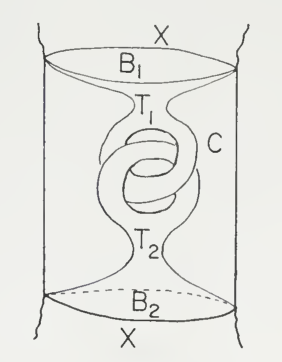
\includegraphics[width=0.5\linewidth]{img mono/hooked rug/3.png}
    \label{hr3}
\end{figure}

\begin{teo}{Teorema 11} Sean $C$ un cubo topológico, $B_1,\; B_2,\; B_3\subset\partial C$ discos disjuntos dos a dos, $C_1$ cubo topológico tal que $C_1\cap int(C)^c =B_1\cup B_2$, $T$ un toro sólido tal que $T\cap C=B_3$ y tal que $T$ engancha $C_1$. 

Sea $X$ un cerrado tal que $X\cap C= B_1\cup B_2\cup B_3$ y tal que $\partial B_i$ no es homotópico a un punto en $\partial B_i \cup (X\cup C)^c$ para $i=1,\;2$. 

Entonces, si $J$ es una curva simple cerrada en $(X\cup C)^c$ y no es homotópica a un punto en $(X\cup C)^c$, se tiene que $J$ no es homotópica a un punto en $(X\cup C_1\cup T)^c$. \end{teo}

\begin{figure}[h!]
    \centering
    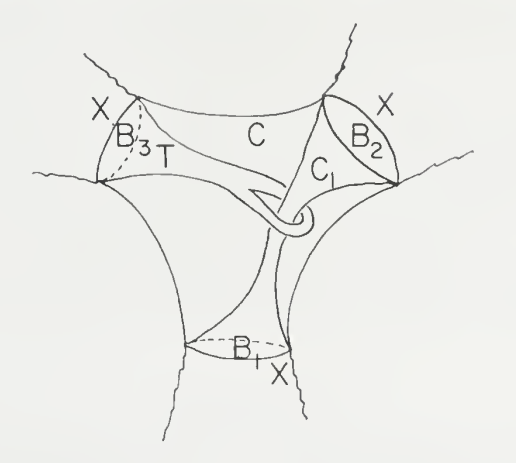
\includegraphics[width=0.5\linewidth]{img mono/hooked rug/4.png}
    \label{hr4}
\end{figure}


\section*{Cronograma}

El trabajo se encuentra en un estado avanzado de desarrollo. Este se entregará al tribunal durante el mes de \textit{febrero}, y será defendido posteriormente en el correr de los meses \textit{febrero-marzo}.

\section*{Tribunal}

\noindent Sugerimos el siguiente tribunal:\\

Richard Muñiz, Aldo Portela y Rafael Potrie. \\

\noindent Suplente: Juliana Xavier (orientadora).

% El siguiente cronograma es tentativo y podrá sufrir modificaciones durante el
% desarrollo de la monografía.\\

% Ya se comenz\'o a trabajar el a\~no pasado habiendo completado el estudio preliminar de la homología simplicial y singular, la sucesión de Mayer--Vietoris, el teorema de
%     Jordan--Brouwer, la relación entre el grupo fundamental y el primer grupo de
%     homología, y el teorema generalizado de Schoenflies.  Lo que sigue es el cronograma para este semestre que comienza y la posterior defensa a fin de a\~no:

% \begin{itemize}


%     \item \textbf{Febrero:} Correcciones finales, entrega al tribunal y preparación de la defensa.
    
%     \item \textbf{Febrero-Marzo:} Defensa.

    
% \end{itemize}

\section*{Bibliografía principal}

\begin{itemize}
    \item A. Hatcher, \emph{Algebraic Topology}.
    \item R. Daverman, G. Venema, \emph{Embeddings in Manifolds}.
    \item T. B. Rushing, \emph{Topological Embeddings}
    % \item S. Mac Lane, \emph{Categories for the Working Mathematician}.
    \item M. Brown, \emph{A Proof of the Generalized Schoenflies Theorem}.
    \item R. Kirby, \emph{On the Set of Non-Locally Flat Points of a Submanifold of Codimension One}.
    \item R. H. Bing, \emph{A Wild Surface Each of Whose Arcs is Tame}.
\end{itemize}

\vspace{2cm}

\begin{flushright}
Micaela Berezan \hfill Orientadora 
\end{flushright}

\end{document}